% **************************************************************************************************************
% A Classic Thesis Style
% An Homage to The Elements of Typographic Style
%
% Copyright (C) 2025 André Miede and Ivo Pletikosić
%
% If you like the style then I would appreciate a postcard. My address
% can be found in the file ClassicThesis.pdf. A collection of the
% postcards I received so far is available online at
% http://postcards.miede.de
%
% License:
% This program is free software; you can redistribute it and/or modify
% it under the terms of the GNU General Public License as published by
% the Free Software Foundation; either version 2 of the License, or
% (at your option) any later version.
%
% This program is distributed in the hope that it will be useful,
% but WITHOUT ANY WARRANTY; without even the implied warranty of
% MERCHANTABILITY or FITNESS FOR A PARTICULAR PURPOSE.  See the
% GNU General Public License for more details.
%
% You should have received a copy of the GNU General Public License
% along with this program; see the file COPYING.  If not, write to
% the Free Software Foundation, Inc., 59 Temple Place - Suite 330,
% Boston, MA 02111-1307, USA.
%
% PLEASE SEE ALSO THE AUTHORS' NOTE REGARDING THIS LICENSE
% IN THE DOCUMENTATION (ClassicThesis.pdf --> Chapter 1 / Chapter01.tex)
% **************************************************************************************************************
\RequirePackage{silence} % :-\
    \WarningFilter{scrreprt}{Usage of package `titlesec'}
    %\WarningFilter{scrreprt}{Activating an ugly workaround}
    \WarningFilter{titlesec}{Non standard sectioning command detected}
\documentclass[ twoside,openright,titlepage,numbers=noenddot,%1headlines,
                headinclude,footinclude,cleardoublepage=empty,abstract=on,
                BCOR=5mm,paper=a4,fontsize=11pt
                ]{scrreprt}

%********************************************************************
% Note: Make all your adjustments in here
%*******************************************************
% ****************************************************************************************************
% classicthesis-config.tex
% formerly known as loadpackages.sty, classicthesis-ldpkg.sty, and classicthesis-preamble.sty
% Use it at the beginning of your ClassicThesis.tex, or as a LaTeX Preamble
% in your ClassicThesis.{tex,lyx} with % ****************************************************************************************************
% classicthesis-config.tex
% formerly known as loadpackages.sty, classicthesis-ldpkg.sty, and classicthesis-preamble.sty
% Use it at the beginning of your ClassicThesis.tex, or as a LaTeX Preamble
% in your ClassicThesis.{tex,lyx} with % ****************************************************************************************************
% classicthesis-config.tex
% formerly known as loadpackages.sty, classicthesis-ldpkg.sty, and classicthesis-preamble.sty
% Use it at the beginning of your ClassicThesis.tex, or as a LaTeX Preamble
% in your ClassicThesis.{tex,lyx} with \input{classicthesis-config}
% ****************************************************************************************************
% If you like the classicthesis, then I would appreciate a postcard.
% My address can be found in the file ClassicThesis.pdf. A collection
% of the postcards I received so far is available online at
% http://postcards.miede.de
% ****************************************************************************************************


% ****************************************************************************************************
% 0. Set the encoding of your files. UTF-8 is the only sensible encoding nowadays. If you can't read
% äöüßáéçèê∂åëæƒÏ€ then change the encoding setting in your editor, not the line below. If your editor
% does not support utf8 use another editor!
% ****************************************************************************************************
\PassOptionsToPackage{utf8}{inputenc}
  \usepackage{inputenc}

\PassOptionsToPackage{T1}{fontenc} % T2A for cyrillics
  \usepackage{fontenc}


% ****************************************************************************************************
% 1. Configure classicthesis for your needs here, e.g., remove "drafting" below
% in order to deactivate the time-stamp on the pages
% (see ClassicThesis.pdf for more information):
% ****************************************************************************************************
\PassOptionsToPackage{
  drafting=false,    % print version information on the bottom of the pages
  tocaligned=false, % the left column of the toc will be aligned (no indentation)
  dottedtoc=false,  % page numbers in ToC flushed right
  eulerchapternumbers=false, % use AMS Euler for chapter font (otherwise Palatino)
  floatperchapter=true,     % numbering per chapter for all floats (i.e., Figure 1.1)
  eulermath=false,  % use awesome Euler fonts for mathematical formulae (only with pdfLaTeX)
  beramono=true,    % toggle a nice monospaced font (w/ bold)
  palatino=true,    % deactivate standard font for loading another one, see the last section at the end of this file for suggestions
  %linedheaders=true, % obsolete / available for backwards compatibility
  style=classicthesis % classicthesis, arsclassica, linedheaders, plain
}{classicthesis}

% ****************************************************************************************************
% 2. Personal data and user ad-hoc commands (insert your own data here)
% ****************************************************************************************************
\newcommand{\myTitle}{Landing in the Latent Space\xspace}
\newcommand{\mySubtitle}{Building Labeled Synthetic Runway Datasets with a Data Augmentation Pipeline that uses Diffusion Models\xspace}
\newcommand{\myDegree}{BSc Computer Science\xspace}
\newcommand{\myName}{Gustavo de Paula\xspace}
\newcommand{\myProf}{Put name here\xspace}
\newcommand{\myOtherProf}{Put name here\xspace}
\newcommand{\mySupervisor}{Put name here\xspace}
\newcommand{\myFaculty}{Put data here\xspace}
\newcommand{\myDepartment}{Computer Science\xspace}
\newcommand{\myUni}{University of London\xspace}
\newcommand{\myLocation}{São Paulo\xspace}
\newcommand{\myTime}{March 2025\xspace}
\newcommand{\myVersion}{\classicthesis}

% ********************************************************************
% Setup, finetuning, and useful commands
% ********************************************************************
\providecommand{\mLyX}{L\kern-.1667em\lower.25em\hbox{Y}\kern-.125emX\@}
\newcommand{\ie}{i.\,e.}
\newcommand{\Ie}{I.\,e.}
\newcommand{\eg}{e.\,g.}
\newcommand{\Eg}{E.\,g.}
% ****************************************************************************************************


% ****************************************************************************************************
% 3. Loading some handy packages
% ****************************************************************************************************
% ********************************************************************
% Packages with options that might require adjustments
% ********************************************************************
\PassOptionsToPackage{american}{babel} % change this to your language(s), main language last
% Spanish languages need extra options in order to work with this template
%\PassOptionsToPackage{spanish,es-lcroman}{babel}
    \usepackage{babel}

\usepackage{csquotes}
\PassOptionsToPackage{%
  %backend=biber,bibencoding=utf8, %instead of bibtex
  backend=bibtex8,bibencoding=auto,% ascii
  language=auto,%
  style=numeric-comp,%
  %style=authoryear-comp, % Author 1999, 2010
  %bibstyle=authoryear,dashed=false, % dashed: substitute rep. author with ---
  sorting=nyt, % name, year, title
  maxbibnames=10, % default: 3, et al.
  %backref=true,%
  natbib=true % natbib compatibility mode (\citep and \citet still work)
}{biblatex}
    \usepackage{biblatex}

\PassOptionsToPackage{fleqn}{amsmath}       % math environments and more by the AMS
  \usepackage{amsmath}

% ********************************************************************
% General useful packages
% ********************************************************************
\usepackage{graphicx} %
\usepackage{scrhack} % fix warnings when using KOMA with listings package
\usepackage{xspace} % to get the spacing after macros right
\PassOptionsToPackage{printonlyused,smaller}{acronym}
  \usepackage{acronym} % nice macros for handling all acronyms in the thesis
  %\renewcommand{\bflabel}[1]{{#1}\hfill} % fix the list of acronyms --> no longer working
  %\renewcommand*{\acsfont}[1]{\textsc{#1}}
  %\renewcommand*{\aclabelfont}[1]{\acsfont{#1}}
  %\def\bflabel#1{{#1\hfill}}
  \def\bflabel#1{{\acsfont{#1}\hfill}}
  \def\aclabelfont#1{\acsfont{#1}}
% ****************************************************************************************************
%\usepackage{pgfplots} % External TikZ/PGF support (thanks to Andreas Nautsch)
%\usetikzlibrary{external}
%\tikzexternalize[mode=list and make, prefix=ext-tikz/]
% ****************************************************************************************************


% ****************************************************************************************************
% 4. Setup floats: tables, (sub)figures, and captions
% ****************************************************************************************************
\usepackage{tabularx} % better tables
  \setlength{\extrarowheight}{3pt} % increase table row height
\newcommand{\tableheadline}[1]{\multicolumn{1}{l}{\spacedlowsmallcaps{#1}}}
\newcommand{\myfloatalign}{\centering} % to be used with each float for alignment
\usepackage{subfig}
% ****************************************************************************************************


% ****************************************************************************************************
% 5. Setup code listings
% ****************************************************************************************************
\usepackage{listings}
%\lstset{emph={trueIndex,root},emphstyle=\color{BlueViolet}}%\underbar} % for special keywords
\lstset{language=[LaTeX]Tex,%C++,
  morekeywords={PassOptionsToPackage,selectlanguage},
  keywordstyle=\color{RoyalBlue},%\bfseries,
  basicstyle=\small\ttfamily,
  %identifierstyle=\color{NavyBlue},
  commentstyle=\color{Green}\ttfamily,
  stringstyle=\rmfamily,
  numbers=none,%left,%
  numberstyle=\scriptsize,%\tiny
  stepnumber=5,
  numbersep=8pt,
  showstringspaces=false,
  breaklines=true,
  %frameround=ftff,
  %frame=single,
  belowcaptionskip=.75\baselineskip
  %frame=L
}

\lstset{
    backgroundcolor=\color{monokai-bg},
    basicstyle=\ttfamily\footnotesize\color{monokai-fg},
    keywordstyle=\color{monokai-purple}\bfseries,
    stringstyle=\color{monokai-green},
    commentstyle=\color{monokai-comment}\itshape,
    numberstyle=\tiny\color{gray},
    numbers=left,
    stepnumber=1,
    numbersep=10pt,
    showstringspaces=false,
    breaklines=true,
    frame=single,
    language=Python
}

\usepackage{placeins}
\usepackage{multirow}
\usepackage{pgfplots}
\usepackage{pgfplots}
\pgfplotsset{compat=1.18}
\usepackage{pgfplotstable}
\usepackage{tikz}
\usepackage{filecontents}
\usepackage[dvipsnames]{xcolor}




% ****************************************************************************************************


% ****************************************************************************************************
% 6. Last calls before the bar closes
% ****************************************************************************************************
% ********************************************************************
% Her Majesty herself
% ********************************************************************
\PassOptionsToPackage{hyperfootnotes=false}{hyperref}
\usepackage{classicthesis}


% ********************************************************************
% Fine-tune hyperreferences (hyperref should be called last)
% ********************************************************************
\hypersetup{%
  %draft, % hyperref's draft mode, for printing see below
  colorlinks=true, linktocpage=true, pdfstartpage=3, pdfstartview=FitV,%
  % uncomment the following line if you want to have black links (e.g., for printing)
  %colorlinks=false, linktocpage=false, pdfstartpage=3, pdfstartview=FitV, pdfborder={0 0 0},%
  breaklinks=true, pageanchor=true,%
  pdfpagemode=UseNone, %
  % pdfpagemode=UseOutlines,%
  plainpages=false, bookmarksnumbered, bookmarksopen=true, bookmarksopenlevel=1,%
  hypertexnames=true, pdfhighlight=/O,%nesting=true,%frenchlinks,%
  urlcolor=CTurl, linkcolor=CTlink, citecolor=CTcitation, %pagecolor=RoyalBlue,%
  %urlcolor=Black, linkcolor=Black, citecolor=Black, %pagecolor=Black,%
  pdftitle={\myTitle},%
  pdfauthor={\textcopyright\ \myName, \myUni, \myFaculty},%
  pdfsubject={},%
  pdfkeywords={},%
  pdfcreator={pdfLaTeX},%
  pdfproducer={LaTeX with hyperref and classicthesis}%
}


% ********************************************************************
% Setup autoreferences (hyperref and babel)
% ********************************************************************
% There are some issues regarding autorefnames
% http://www.tex.ac.uk/cgi-bin/texfaq2html?label=latexwords
% you have to redefine the macros for the
% language you use, e.g., american, ngerman
% (as chosen when loading babel/AtBeginDocument)
% ********************************************************************
 \makeatletter
 \@ifpackageloaded{babel}%
   {%
     \addto\extrasamerican{%
       \renewcommand*{\figureautorefname}{Figure}%
       \renewcommand*{\tableautorefname}{Table}%
       \renewcommand*{\partautorefname}{Part}%
       \renewcommand*{\chapterautorefname}{Chapter}%
       \renewcommand*{\sectionautorefname}{Section}%
       \renewcommand*{\subsectionautorefname}{Section}%
       \renewcommand*{\subsubsectionautorefname}{Section}%
     }%
     % \addto\extrasngerman{%
     %   \renewcommand*{\paragraphautorefname}{Absatz}%
     %   \renewcommand*{\subparagraphautorefname}{Unterabsatz}%
     %   \renewcommand*{\footnoteautorefname}{Fu\"snote}%
     %   \renewcommand*{\FancyVerbLineautorefname}{Zeile}%
     %   \renewcommand*{\theoremautorefname}{Theorem}%
     %   \renewcommand*{\appendixautorefname}{Anhang}%
     %   \renewcommand*{\equationautorefname}{Gleichung}%
     %   \renewcommand*{\itemautorefname}{Punkt}%
     % }%
       % Fix to getting autorefs for subfigures right (thanks to Belinda Vogt for changing the definition)
       \providecommand{\subfigureautorefname}{\figureautorefname}%
     }{\relax}
 \makeatother

% (Better) alternative to \autoref is \cref via the cleveref package
%\usepackage{cleveref}
%\crefformat{part}{Part #2\MakeUppercase{#1}#3}


% ********************************************************************
% Development Stuff
% ********************************************************************
\listfiles
%\PassOptionsToPackage{l2tabu,orthodox,abort}{nag}
%  \usepackage{nag}
%\PassOptionsToPackage{warning, all}{onlyamsmath}
%  \usepackage{onlyamsmath}


% ****************************************************************************************************
% 7. Further adjustments (experimental)
% ****************************************************************************************************
% ********************************************************************
% Changing the text area
% ********************************************************************
%\areaset[current]{312pt}{761pt} % 686 (factor 2.2) + 33 head + 42 head \the\footskip
%\setlength{\marginparwidth}{7em}%
%\setlength{\marginparsep}{2em}%

% ********************************************************************
% Using different fonts
% ********************************************************************
%\usepackage[oldstylenums]{kpfonts} % oldstyle notextcomp
% \usepackage[osf]{libertine}
%\usepackage[light,condensed,math]{iwona}
%\renewcommand{\sfdefault}{iwona}
%\usepackage{lmodern} % <-- no osf support :-(
%\usepackage{cfr-lm} %
%\usepackage[urw-garamond]{mathdesign} <-- no osf support :-(
%\usepackage[default,osfigures]{opensans} % scale=0.95
%\usepackage[sfdefault]{FiraSans}
% \usepackage[opticals,mathlf]{MinionPro} % onlytext
% ********************************************************************
%\usepackage[largesc,osf]{newpxtext}
%\linespread{1.05} % a bit more for Palatino
% Used to fix these:
% https://bitbucket.org/amiede/classicthesis/issues/139/italics-in-pallatino-capitals-chapter
% https://bitbucket.org/amiede/classicthesis/issues/45/problema-testatine-su-classicthesis-style
% ********************************************************************
% ****************************************************************************************************

% ****************************************************************************************************
% If you like the classicthesis, then I would appreciate a postcard.
% My address can be found in the file ClassicThesis.pdf. A collection
% of the postcards I received so far is available online at
% http://postcards.miede.de
% ****************************************************************************************************


% ****************************************************************************************************
% 0. Set the encoding of your files. UTF-8 is the only sensible encoding nowadays. If you can't read
% äöüßáéçèê∂åëæƒÏ€ then change the encoding setting in your editor, not the line below. If your editor
% does not support utf8 use another editor!
% ****************************************************************************************************
\PassOptionsToPackage{utf8}{inputenc}
  \usepackage{inputenc}

\PassOptionsToPackage{T1}{fontenc} % T2A for cyrillics
  \usepackage{fontenc}


% ****************************************************************************************************
% 1. Configure classicthesis for your needs here, e.g., remove "drafting" below
% in order to deactivate the time-stamp on the pages
% (see ClassicThesis.pdf for more information):
% ****************************************************************************************************
\PassOptionsToPackage{
  drafting=false,    % print version information on the bottom of the pages
  tocaligned=false, % the left column of the toc will be aligned (no indentation)
  dottedtoc=false,  % page numbers in ToC flushed right
  eulerchapternumbers=false, % use AMS Euler for chapter font (otherwise Palatino)
  floatperchapter=true,     % numbering per chapter for all floats (i.e., Figure 1.1)
  eulermath=false,  % use awesome Euler fonts for mathematical formulae (only with pdfLaTeX)
  beramono=true,    % toggle a nice monospaced font (w/ bold)
  palatino=true,    % deactivate standard font for loading another one, see the last section at the end of this file for suggestions
  %linedheaders=true, % obsolete / available for backwards compatibility
  style=classicthesis % classicthesis, arsclassica, linedheaders, plain
}{classicthesis}

% ****************************************************************************************************
% 2. Personal data and user ad-hoc commands (insert your own data here)
% ****************************************************************************************************
\newcommand{\myTitle}{Landing in the Latent Space\xspace}
\newcommand{\mySubtitle}{Building Labeled Synthetic Runway Datasets with a Data Augmentation Pipeline that uses Diffusion Models\xspace}
\newcommand{\myDegree}{BSc Computer Science\xspace}
\newcommand{\myName}{Gustavo de Paula\xspace}
\newcommand{\myProf}{Put name here\xspace}
\newcommand{\myOtherProf}{Put name here\xspace}
\newcommand{\mySupervisor}{Put name here\xspace}
\newcommand{\myFaculty}{Put data here\xspace}
\newcommand{\myDepartment}{Computer Science\xspace}
\newcommand{\myUni}{University of London\xspace}
\newcommand{\myLocation}{São Paulo\xspace}
\newcommand{\myTime}{March 2025\xspace}
\newcommand{\myVersion}{\classicthesis}

% ********************************************************************
% Setup, finetuning, and useful commands
% ********************************************************************
\providecommand{\mLyX}{L\kern-.1667em\lower.25em\hbox{Y}\kern-.125emX\@}
\newcommand{\ie}{i.\,e.}
\newcommand{\Ie}{I.\,e.}
\newcommand{\eg}{e.\,g.}
\newcommand{\Eg}{E.\,g.}
% ****************************************************************************************************


% ****************************************************************************************************
% 3. Loading some handy packages
% ****************************************************************************************************
% ********************************************************************
% Packages with options that might require adjustments
% ********************************************************************
\PassOptionsToPackage{american}{babel} % change this to your language(s), main language last
% Spanish languages need extra options in order to work with this template
%\PassOptionsToPackage{spanish,es-lcroman}{babel}
    \usepackage{babel}

\usepackage{csquotes}
\PassOptionsToPackage{%
  %backend=biber,bibencoding=utf8, %instead of bibtex
  backend=bibtex8,bibencoding=auto,% ascii
  language=auto,%
  style=numeric-comp,%
  %style=authoryear-comp, % Author 1999, 2010
  %bibstyle=authoryear,dashed=false, % dashed: substitute rep. author with ---
  sorting=nyt, % name, year, title
  maxbibnames=10, % default: 3, et al.
  %backref=true,%
  natbib=true % natbib compatibility mode (\citep and \citet still work)
}{biblatex}
    \usepackage{biblatex}

\PassOptionsToPackage{fleqn}{amsmath}       % math environments and more by the AMS
  \usepackage{amsmath}

% ********************************************************************
% General useful packages
% ********************************************************************
\usepackage{graphicx} %
\usepackage{scrhack} % fix warnings when using KOMA with listings package
\usepackage{xspace} % to get the spacing after macros right
\PassOptionsToPackage{printonlyused,smaller}{acronym}
  \usepackage{acronym} % nice macros for handling all acronyms in the thesis
  %\renewcommand{\bflabel}[1]{{#1}\hfill} % fix the list of acronyms --> no longer working
  %\renewcommand*{\acsfont}[1]{\textsc{#1}}
  %\renewcommand*{\aclabelfont}[1]{\acsfont{#1}}
  %\def\bflabel#1{{#1\hfill}}
  \def\bflabel#1{{\acsfont{#1}\hfill}}
  \def\aclabelfont#1{\acsfont{#1}}
% ****************************************************************************************************
%\usepackage{pgfplots} % External TikZ/PGF support (thanks to Andreas Nautsch)
%\usetikzlibrary{external}
%\tikzexternalize[mode=list and make, prefix=ext-tikz/]
% ****************************************************************************************************


% ****************************************************************************************************
% 4. Setup floats: tables, (sub)figures, and captions
% ****************************************************************************************************
\usepackage{tabularx} % better tables
  \setlength{\extrarowheight}{3pt} % increase table row height
\newcommand{\tableheadline}[1]{\multicolumn{1}{l}{\spacedlowsmallcaps{#1}}}
\newcommand{\myfloatalign}{\centering} % to be used with each float for alignment
\usepackage{subfig}
% ****************************************************************************************************


% ****************************************************************************************************
% 5. Setup code listings
% ****************************************************************************************************
\usepackage{listings}
%\lstset{emph={trueIndex,root},emphstyle=\color{BlueViolet}}%\underbar} % for special keywords
\lstset{language=[LaTeX]Tex,%C++,
  morekeywords={PassOptionsToPackage,selectlanguage},
  keywordstyle=\color{RoyalBlue},%\bfseries,
  basicstyle=\small\ttfamily,
  %identifierstyle=\color{NavyBlue},
  commentstyle=\color{Green}\ttfamily,
  stringstyle=\rmfamily,
  numbers=none,%left,%
  numberstyle=\scriptsize,%\tiny
  stepnumber=5,
  numbersep=8pt,
  showstringspaces=false,
  breaklines=true,
  %frameround=ftff,
  %frame=single,
  belowcaptionskip=.75\baselineskip
  %frame=L
}

\lstset{
    backgroundcolor=\color{monokai-bg},
    basicstyle=\ttfamily\footnotesize\color{monokai-fg},
    keywordstyle=\color{monokai-purple}\bfseries,
    stringstyle=\color{monokai-green},
    commentstyle=\color{monokai-comment}\itshape,
    numberstyle=\tiny\color{gray},
    numbers=left,
    stepnumber=1,
    numbersep=10pt,
    showstringspaces=false,
    breaklines=true,
    frame=single,
    language=Python
}

\usepackage{placeins}
\usepackage{multirow}
\usepackage{pgfplots}
\usepackage{pgfplots}
\pgfplotsset{compat=1.18}
\usepackage{pgfplotstable}
\usepackage{tikz}
\usepackage{filecontents}
\usepackage[dvipsnames]{xcolor}




% ****************************************************************************************************


% ****************************************************************************************************
% 6. Last calls before the bar closes
% ****************************************************************************************************
% ********************************************************************
% Her Majesty herself
% ********************************************************************
\PassOptionsToPackage{hyperfootnotes=false}{hyperref}
\usepackage{classicthesis}


% ********************************************************************
% Fine-tune hyperreferences (hyperref should be called last)
% ********************************************************************
\hypersetup{%
  %draft, % hyperref's draft mode, for printing see below
  colorlinks=true, linktocpage=true, pdfstartpage=3, pdfstartview=FitV,%
  % uncomment the following line if you want to have black links (e.g., for printing)
  %colorlinks=false, linktocpage=false, pdfstartpage=3, pdfstartview=FitV, pdfborder={0 0 0},%
  breaklinks=true, pageanchor=true,%
  pdfpagemode=UseNone, %
  % pdfpagemode=UseOutlines,%
  plainpages=false, bookmarksnumbered, bookmarksopen=true, bookmarksopenlevel=1,%
  hypertexnames=true, pdfhighlight=/O,%nesting=true,%frenchlinks,%
  urlcolor=CTurl, linkcolor=CTlink, citecolor=CTcitation, %pagecolor=RoyalBlue,%
  %urlcolor=Black, linkcolor=Black, citecolor=Black, %pagecolor=Black,%
  pdftitle={\myTitle},%
  pdfauthor={\textcopyright\ \myName, \myUni, \myFaculty},%
  pdfsubject={},%
  pdfkeywords={},%
  pdfcreator={pdfLaTeX},%
  pdfproducer={LaTeX with hyperref and classicthesis}%
}


% ********************************************************************
% Setup autoreferences (hyperref and babel)
% ********************************************************************
% There are some issues regarding autorefnames
% http://www.tex.ac.uk/cgi-bin/texfaq2html?label=latexwords
% you have to redefine the macros for the
% language you use, e.g., american, ngerman
% (as chosen when loading babel/AtBeginDocument)
% ********************************************************************
 \makeatletter
 \@ifpackageloaded{babel}%
   {%
     \addto\extrasamerican{%
       \renewcommand*{\figureautorefname}{Figure}%
       \renewcommand*{\tableautorefname}{Table}%
       \renewcommand*{\partautorefname}{Part}%
       \renewcommand*{\chapterautorefname}{Chapter}%
       \renewcommand*{\sectionautorefname}{Section}%
       \renewcommand*{\subsectionautorefname}{Section}%
       \renewcommand*{\subsubsectionautorefname}{Section}%
     }%
     % \addto\extrasngerman{%
     %   \renewcommand*{\paragraphautorefname}{Absatz}%
     %   \renewcommand*{\subparagraphautorefname}{Unterabsatz}%
     %   \renewcommand*{\footnoteautorefname}{Fu\"snote}%
     %   \renewcommand*{\FancyVerbLineautorefname}{Zeile}%
     %   \renewcommand*{\theoremautorefname}{Theorem}%
     %   \renewcommand*{\appendixautorefname}{Anhang}%
     %   \renewcommand*{\equationautorefname}{Gleichung}%
     %   \renewcommand*{\itemautorefname}{Punkt}%
     % }%
       % Fix to getting autorefs for subfigures right (thanks to Belinda Vogt for changing the definition)
       \providecommand{\subfigureautorefname}{\figureautorefname}%
     }{\relax}
 \makeatother

% (Better) alternative to \autoref is \cref via the cleveref package
%\usepackage{cleveref}
%\crefformat{part}{Part #2\MakeUppercase{#1}#3}


% ********************************************************************
% Development Stuff
% ********************************************************************
\listfiles
%\PassOptionsToPackage{l2tabu,orthodox,abort}{nag}
%  \usepackage{nag}
%\PassOptionsToPackage{warning, all}{onlyamsmath}
%  \usepackage{onlyamsmath}


% ****************************************************************************************************
% 7. Further adjustments (experimental)
% ****************************************************************************************************
% ********************************************************************
% Changing the text area
% ********************************************************************
%\areaset[current]{312pt}{761pt} % 686 (factor 2.2) + 33 head + 42 head \the\footskip
%\setlength{\marginparwidth}{7em}%
%\setlength{\marginparsep}{2em}%

% ********************************************************************
% Using different fonts
% ********************************************************************
%\usepackage[oldstylenums]{kpfonts} % oldstyle notextcomp
% \usepackage[osf]{libertine}
%\usepackage[light,condensed,math]{iwona}
%\renewcommand{\sfdefault}{iwona}
%\usepackage{lmodern} % <-- no osf support :-(
%\usepackage{cfr-lm} %
%\usepackage[urw-garamond]{mathdesign} <-- no osf support :-(
%\usepackage[default,osfigures]{opensans} % scale=0.95
%\usepackage[sfdefault]{FiraSans}
% \usepackage[opticals,mathlf]{MinionPro} % onlytext
% ********************************************************************
%\usepackage[largesc,osf]{newpxtext}
%\linespread{1.05} % a bit more for Palatino
% Used to fix these:
% https://bitbucket.org/amiede/classicthesis/issues/139/italics-in-pallatino-capitals-chapter
% https://bitbucket.org/amiede/classicthesis/issues/45/problema-testatine-su-classicthesis-style
% ********************************************************************
% ****************************************************************************************************

% ****************************************************************************************************
% If you like the classicthesis, then I would appreciate a postcard.
% My address can be found in the file ClassicThesis.pdf. A collection
% of the postcards I received so far is available online at
% http://postcards.miede.de
% ****************************************************************************************************


% ****************************************************************************************************
% 0. Set the encoding of your files. UTF-8 is the only sensible encoding nowadays. If you can't read
% äöüßáéçèê∂åëæƒÏ€ then change the encoding setting in your editor, not the line below. If your editor
% does not support utf8 use another editor!
% ****************************************************************************************************
\PassOptionsToPackage{utf8}{inputenc}
  \usepackage{inputenc}

\PassOptionsToPackage{T1}{fontenc} % T2A for cyrillics
  \usepackage{fontenc}


% ****************************************************************************************************
% 1. Configure classicthesis for your needs here, e.g., remove "drafting" below
% in order to deactivate the time-stamp on the pages
% (see ClassicThesis.pdf for more information):
% ****************************************************************************************************
\PassOptionsToPackage{
  drafting=false,    % print version information on the bottom of the pages
  tocaligned=false, % the left column of the toc will be aligned (no indentation)
  dottedtoc=false,  % page numbers in ToC flushed right
  eulerchapternumbers=false, % use AMS Euler for chapter font (otherwise Palatino)
  floatperchapter=true,     % numbering per chapter for all floats (i.e., Figure 1.1)
  eulermath=false,  % use awesome Euler fonts for mathematical formulae (only with pdfLaTeX)
  beramono=true,    % toggle a nice monospaced font (w/ bold)
  palatino=true,    % deactivate standard font for loading another one, see the last section at the end of this file for suggestions
  %linedheaders=true, % obsolete / available for backwards compatibility
  style=classicthesis % classicthesis, arsclassica, linedheaders, plain
}{classicthesis}

% ****************************************************************************************************
% 2. Personal data and user ad-hoc commands (insert your own data here)
% ****************************************************************************************************
\newcommand{\myTitle}{Landing in the Latent Space\xspace}
\newcommand{\mySubtitle}{Building Labeled Synthetic Runway Datasets with a Data Augmentation Pipeline that uses Diffusion Models\xspace}
\newcommand{\myDegree}{BSc Computer Science\xspace}
\newcommand{\myName}{Gustavo de Paula\xspace}
\newcommand{\myProf}{Put name here\xspace}
\newcommand{\myOtherProf}{Put name here\xspace}
\newcommand{\mySupervisor}{Put name here\xspace}
\newcommand{\myFaculty}{Put data here\xspace}
\newcommand{\myDepartment}{Computer Science\xspace}
\newcommand{\myUni}{University of London\xspace}
\newcommand{\myLocation}{São Paulo\xspace}
\newcommand{\myTime}{March 2025\xspace}
\newcommand{\myVersion}{\classicthesis}

% ********************************************************************
% Setup, finetuning, and useful commands
% ********************************************************************
\providecommand{\mLyX}{L\kern-.1667em\lower.25em\hbox{Y}\kern-.125emX\@}
\newcommand{\ie}{i.\,e.}
\newcommand{\Ie}{I.\,e.}
\newcommand{\eg}{e.\,g.}
\newcommand{\Eg}{E.\,g.}
% ****************************************************************************************************


% ****************************************************************************************************
% 3. Loading some handy packages
% ****************************************************************************************************
% ********************************************************************
% Packages with options that might require adjustments
% ********************************************************************
\PassOptionsToPackage{american}{babel} % change this to your language(s), main language last
% Spanish languages need extra options in order to work with this template
%\PassOptionsToPackage{spanish,es-lcroman}{babel}
    \usepackage{babel}

\usepackage{csquotes}
\PassOptionsToPackage{%
  %backend=biber,bibencoding=utf8, %instead of bibtex
  backend=bibtex8,bibencoding=auto,% ascii
  language=auto,%
  style=numeric-comp,%
  %style=authoryear-comp, % Author 1999, 2010
  %bibstyle=authoryear,dashed=false, % dashed: substitute rep. author with ---
  sorting=nyt, % name, year, title
  maxbibnames=10, % default: 3, et al.
  %backref=true,%
  natbib=true % natbib compatibility mode (\citep and \citet still work)
}{biblatex}
    \usepackage{biblatex}

\PassOptionsToPackage{fleqn}{amsmath}       % math environments and more by the AMS
  \usepackage{amsmath}

% ********************************************************************
% General useful packages
% ********************************************************************
\usepackage{graphicx} %
\usepackage{scrhack} % fix warnings when using KOMA with listings package
\usepackage{xspace} % to get the spacing after macros right
\PassOptionsToPackage{printonlyused,smaller}{acronym}
  \usepackage{acronym} % nice macros for handling all acronyms in the thesis
  %\renewcommand{\bflabel}[1]{{#1}\hfill} % fix the list of acronyms --> no longer working
  %\renewcommand*{\acsfont}[1]{\textsc{#1}}
  %\renewcommand*{\aclabelfont}[1]{\acsfont{#1}}
  %\def\bflabel#1{{#1\hfill}}
  \def\bflabel#1{{\acsfont{#1}\hfill}}
  \def\aclabelfont#1{\acsfont{#1}}
% ****************************************************************************************************
%\usepackage{pgfplots} % External TikZ/PGF support (thanks to Andreas Nautsch)
%\usetikzlibrary{external}
%\tikzexternalize[mode=list and make, prefix=ext-tikz/]
% ****************************************************************************************************


% ****************************************************************************************************
% 4. Setup floats: tables, (sub)figures, and captions
% ****************************************************************************************************
\usepackage{tabularx} % better tables
  \setlength{\extrarowheight}{3pt} % increase table row height
\newcommand{\tableheadline}[1]{\multicolumn{1}{l}{\spacedlowsmallcaps{#1}}}
\newcommand{\myfloatalign}{\centering} % to be used with each float for alignment
\usepackage{subfig}
% ****************************************************************************************************


% ****************************************************************************************************
% 5. Setup code listings
% ****************************************************************************************************
\usepackage{listings}
%\lstset{emph={trueIndex,root},emphstyle=\color{BlueViolet}}%\underbar} % for special keywords
\lstset{language=[LaTeX]Tex,%C++,
  morekeywords={PassOptionsToPackage,selectlanguage},
  keywordstyle=\color{RoyalBlue},%\bfseries,
  basicstyle=\small\ttfamily,
  %identifierstyle=\color{NavyBlue},
  commentstyle=\color{Green}\ttfamily,
  stringstyle=\rmfamily,
  numbers=none,%left,%
  numberstyle=\scriptsize,%\tiny
  stepnumber=5,
  numbersep=8pt,
  showstringspaces=false,
  breaklines=true,
  %frameround=ftff,
  %frame=single,
  belowcaptionskip=.75\baselineskip
  %frame=L
}

\lstset{
    backgroundcolor=\color{monokai-bg},
    basicstyle=\ttfamily\footnotesize\color{monokai-fg},
    keywordstyle=\color{monokai-purple}\bfseries,
    stringstyle=\color{monokai-green},
    commentstyle=\color{monokai-comment}\itshape,
    numberstyle=\tiny\color{gray},
    numbers=left,
    stepnumber=1,
    numbersep=10pt,
    showstringspaces=false,
    breaklines=true,
    frame=single,
    language=Python
}

\usepackage{placeins}
\usepackage{multirow}
\usepackage{pgfplots}
\usepackage{pgfplots}
\pgfplotsset{compat=1.18}
\usepackage{pgfplotstable}
\usepackage{tikz}
\usepackage{filecontents}
\usepackage[dvipsnames]{xcolor}




% ****************************************************************************************************


% ****************************************************************************************************
% 6. Last calls before the bar closes
% ****************************************************************************************************
% ********************************************************************
% Her Majesty herself
% ********************************************************************
\PassOptionsToPackage{hyperfootnotes=false}{hyperref}
\usepackage{classicthesis}


% ********************************************************************
% Fine-tune hyperreferences (hyperref should be called last)
% ********************************************************************
\hypersetup{%
  %draft, % hyperref's draft mode, for printing see below
  colorlinks=true, linktocpage=true, pdfstartpage=3, pdfstartview=FitV,%
  % uncomment the following line if you want to have black links (e.g., for printing)
  %colorlinks=false, linktocpage=false, pdfstartpage=3, pdfstartview=FitV, pdfborder={0 0 0},%
  breaklinks=true, pageanchor=true,%
  pdfpagemode=UseNone, %
  % pdfpagemode=UseOutlines,%
  plainpages=false, bookmarksnumbered, bookmarksopen=true, bookmarksopenlevel=1,%
  hypertexnames=true, pdfhighlight=/O,%nesting=true,%frenchlinks,%
  urlcolor=CTurl, linkcolor=CTlink, citecolor=CTcitation, %pagecolor=RoyalBlue,%
  %urlcolor=Black, linkcolor=Black, citecolor=Black, %pagecolor=Black,%
  pdftitle={\myTitle},%
  pdfauthor={\textcopyright\ \myName, \myUni, \myFaculty},%
  pdfsubject={},%
  pdfkeywords={},%
  pdfcreator={pdfLaTeX},%
  pdfproducer={LaTeX with hyperref and classicthesis}%
}


% ********************************************************************
% Setup autoreferences (hyperref and babel)
% ********************************************************************
% There are some issues regarding autorefnames
% http://www.tex.ac.uk/cgi-bin/texfaq2html?label=latexwords
% you have to redefine the macros for the
% language you use, e.g., american, ngerman
% (as chosen when loading babel/AtBeginDocument)
% ********************************************************************
 \makeatletter
 \@ifpackageloaded{babel}%
   {%
     \addto\extrasamerican{%
       \renewcommand*{\figureautorefname}{Figure}%
       \renewcommand*{\tableautorefname}{Table}%
       \renewcommand*{\partautorefname}{Part}%
       \renewcommand*{\chapterautorefname}{Chapter}%
       \renewcommand*{\sectionautorefname}{Section}%
       \renewcommand*{\subsectionautorefname}{Section}%
       \renewcommand*{\subsubsectionautorefname}{Section}%
     }%
     % \addto\extrasngerman{%
     %   \renewcommand*{\paragraphautorefname}{Absatz}%
     %   \renewcommand*{\subparagraphautorefname}{Unterabsatz}%
     %   \renewcommand*{\footnoteautorefname}{Fu\"snote}%
     %   \renewcommand*{\FancyVerbLineautorefname}{Zeile}%
     %   \renewcommand*{\theoremautorefname}{Theorem}%
     %   \renewcommand*{\appendixautorefname}{Anhang}%
     %   \renewcommand*{\equationautorefname}{Gleichung}%
     %   \renewcommand*{\itemautorefname}{Punkt}%
     % }%
       % Fix to getting autorefs for subfigures right (thanks to Belinda Vogt for changing the definition)
       \providecommand{\subfigureautorefname}{\figureautorefname}%
     }{\relax}
 \makeatother

% (Better) alternative to \autoref is \cref via the cleveref package
%\usepackage{cleveref}
%\crefformat{part}{Part #2\MakeUppercase{#1}#3}


% ********************************************************************
% Development Stuff
% ********************************************************************
\listfiles
%\PassOptionsToPackage{l2tabu,orthodox,abort}{nag}
%  \usepackage{nag}
%\PassOptionsToPackage{warning, all}{onlyamsmath}
%  \usepackage{onlyamsmath}


% ****************************************************************************************************
% 7. Further adjustments (experimental)
% ****************************************************************************************************
% ********************************************************************
% Changing the text area
% ********************************************************************
%\areaset[current]{312pt}{761pt} % 686 (factor 2.2) + 33 head + 42 head \the\footskip
%\setlength{\marginparwidth}{7em}%
%\setlength{\marginparsep}{2em}%

% ********************************************************************
% Using different fonts
% ********************************************************************
%\usepackage[oldstylenums]{kpfonts} % oldstyle notextcomp
% \usepackage[osf]{libertine}
%\usepackage[light,condensed,math]{iwona}
%\renewcommand{\sfdefault}{iwona}
%\usepackage{lmodern} % <-- no osf support :-(
%\usepackage{cfr-lm} %
%\usepackage[urw-garamond]{mathdesign} <-- no osf support :-(
%\usepackage[default,osfigures]{opensans} % scale=0.95
%\usepackage[sfdefault]{FiraSans}
% \usepackage[opticals,mathlf]{MinionPro} % onlytext
% ********************************************************************
%\usepackage[largesc,osf]{newpxtext}
%\linespread{1.05} % a bit more for Palatino
% Used to fix these:
% https://bitbucket.org/amiede/classicthesis/issues/139/italics-in-pallatino-capitals-chapter
% https://bitbucket.org/amiede/classicthesis/issues/45/problema-testatine-su-classicthesis-style
% ********************************************************************
% ****************************************************************************************************



%********************************************************************
% Bibliographies
%*******************************************************
\addbibresource{Bibliography.bib}
% \addbibresource[label=ownpubs]{AMiede_Publications.bib}

%********************************************************************
% Hyphenation
%*******************************************************
%\hyphenation{put special hyphenation here}

% ********************************************************************
% GO!GO!GO! MOVE IT!
%*******************************************************
\begin{document}
\frenchspacing
\raggedbottom
\selectlanguage{american} % american ngerman
%\renewcommand*{\bibname}{new name}
%\setbibpreamble{}
\pagenumbering{roman}
\pagestyle{plain}
%********************************************************************
% Frontmatter
%*******************************************************
% %*******************************************************
% Little Dirty Titlepage
%*******************************************************
\thispagestyle{empty}
%\pdfbookmark[1]{Titel}{title}
%*******************************************************
\begin{center}
    \spacedlowsmallcaps{\myName} \\ \medskip

    \begingroup
        \color{CTtitle}\spacedallcaps{\myTitle}
    \endgroup
\end{center}

%*******************************************************
% Titlepage
%*******************************************************
\begin{titlepage}
    %\pdfbookmark[1]{\myTitle}{titlepage}
    % if you want the titlepage to be centered, uncomment and fine-tune the line below (KOMA classes environment)
    \begin{addmargin}[-1cm]{-3cm}
    \begin{center}
        \large

        \hfill

        \vfill

        \begingroup
            \color{CTtitle}{\LARGE \spacedallcaps{\myTitle}} \\ \bigskip
        \endgroup

        \spacedlowsmallcaps{\mySubtitle} \\ \bigskip

        \begingroup
          \color{CTtitle}\spacedallcaps{by} \\ \bigskip
        \endgroup

        \spacedallcaps{\large \myName}

        %\includegraphics[width=6cm]{gfx/TFZsuperellipse_bw} \\ \medskip


        \vfill

        
        \vspace{2em}
        Submitted to the Department of \myDepartment\\
        in partial fulfillment of the requirements for the degree of\\[1em]
        \spacedallcaps{\myDegree}\\[0.5em]
        at the\\[0.5em]
        \spacedallcaps{\myUni}\\[1em]

        \myTime

        \vfill

    \end{center}
  \end{addmargin}
\end{titlepage}

\thispagestyle{empty}

\hfill

\vfill

\noindent\myName: \textit{\myTitle,} \mySubtitle, %\myDegree,
\textcopyright\ \myTime

%\bigskip
%
%\noindent\spacedlowsmallcaps{Supervisors}: \\
%\myProf \\
%\myOtherProf \\
%\mySupervisor
%
%\medskip
%
%\noindent\spacedlowsmallcaps{Location}: \\
%\myLocation
%
%\medskip
%
%\noindent\spacedlowsmallcaps{Time Frame}: \\
%\myTime

%*******************************************************
% Dedication
%*******************************************************
\thispagestyle{empty}
\phantomsection
\pdfbookmark[1]{Dedication}{Dedication}

\vspace*{3cm}

\begin{center}
    \emph{"But test everything; hold fast what is good."} \\ \medskip
    --- Saint Paul, First Letter to the Thessalonians 5:21
\end{center}

\medskip

\begin{center}
    This work is dedicated \\ \medskip
    To \emph{Our Lady, Mary}, Mother of God and my mother, in gratitude for
    her maternal care and intercession throughout this journey. \\ \medskip
    
    To \emph{Saint Thomas Aquinas}, the Angelic Doctor, whose love of
    truth shaped the Christian intellectual tradition.
\end{center}


\cleardoublepage%*******************************************************
% Acknowledgments
%*******************************************************
\pdfbookmark[1]{Acknowledgments}{acknowledgments}

\begin{flushright}{\slshape
  Among all human pursuits, the pursuit of wisdom is more \\
  perfect, more noble, more useful, and more full of joy. \medskip

  --- St. Thomas Aquinas \\
  (Summa Contra Gentiles, Book I, Chapter 2)}
  \\ \medskip
\end{flushright}



\bigskip

\begingroup
\let\clearpage\relax
\let\cleardoublepage\relax
\let\cleardoublepage\relax
\chapter*{Acknowledgments}

Above all, I give thanks and praise to Almighty God,
the Most Holy Trinity, without whom nothing has meaning,
and without whose grace this journey would not have been possible.

To the Father, source of all life and providence, for
sustaining me each day. To Jesus Christ, my Savior and
Redeemer, for His mercy and love. To the Holy Spirit,
the Sanctifier, for shining light into the twofold darkness
I was born into: sin and ignorance.

\bigskip

To my father, Heberth de Paula, who has always been a model of
academic excellence and intellectual curiosity, and who has
endured great hardships and sacrifices to provide me
with the best education possible.

\bigskip

To my dearest, my love, and my sweetheart, Júlia de Paula, my
faithful companion, whose love have been the most precious
gift I've received in this passing world.

\bigskip

To my family, friends, work colleagues, and teachers, who
have supported me in countless ways, and who have always
believed in my potential.

\bigskip

To my former employer, Loggi, for taking a chance on me at 17
and investing in my growth—both as an engineer and a student—and
whose financial support enabled me to pursue and complete this
degree. I’m especially grateful to Davi de Castro Reis, who
incentivized me to pursue a degree in Computer Science and
whose support and decision enabled that investment on my education.

\bigskip

\centerline{\textcolor{gray}{\rule{6cm}{0.4pt}}}


\bigskip

\emph{May this work, in whatever good it contains, be for
the glory of God and the service of truth.}

\bigskip


\endgroup

%\cleardoublepage\include{FrontBackmatter/Foreword}
\cleardoublepage%*******************************************************
% Abstract
%*******************************************************
%\renewcommand{\abstractname}{Abstract}
\pdfbookmark[1]{Abstract}{Abstract}
% \addcontentsline{toc}{chapter}{\tocEntry{Abstract}}
\begingroup
% \let\clearpage\relax
% \let\cleardoublepage\relax
% \let\cleardoublepage\relax

\chapter*{Abstract}

Vision-based landing systems have gained increased attention as cost-effective and autonomous alternatives 
to traditional radio-based autoland systems, particularly in scenarios where on-ground infrastructure is 
unavailable or infeasible. A major bottleneck in advancing this technology is the lack of large-scale, diverse, 
and realistic runway image datasets with pixel-level annotations. While recent works have turned to synthetic 
data generated from flight simulators, these approaches are limited by their lack of scalability, poor 
environmental variability, and the high cost of manual annotation.

This paper introduces a novel, open-source, modular data augmentation pipeline, called \emph{Canny2Concrete}, 
that leverages latent diffusion models with ControlNet to generate high-resolution, labeled runway images. 
By conditioning image generation on structural features extracted from existing datasets, the pipeline produces 
realistic synthetic images that preserve critical runway geometry while offering substantial diversity in terms 
of weather, lighting, and background scenery. A three-stage variant generation process enhances image variety 
through positional transformations, outpainting, and environmental occlusion effects.

Using this pipeline, a large-scale synthetic runway dataset---\emph{GARD: Gustavo's Awesome Runway Dataset}---has 
been constructed and evaluated both intrinsically, using the Structural Similarity Index (SSIM), and extrinsically, 
by training and fine-tuning state-of-the-art detection and segmentation models. Results demonstrate that models 
trained on the proposed dataset match or outperform those trained on existing synthetic datasets, confirming 
the viability of diffusion-based augmentation for runway segmentation tasks, and the effectiveness of the
\emph{Canny2Concrete} pipeline in generating realistic runway images. The complete dataset, pipeline, and 
evaluation tools are publicly available to support further research in autonomous aviation and computer vision.

Up to the best of the author's knowledge, and up to date with the literature review conducted in this paper,
\emph{GARD} is the largest synthetic runway dataset publicly available, comprising 45,486 images with diverse
weather, lighting, background, and runway occlusion conditions.

\emph{GARD}, along with trained segmentation model weights and evaluation results, is available at:
\begin{center}
\url{https://www.kaggle.com/datasets/depaulagu/gard2025}
\end{center}

The code for the project, including the implementation of the \emph{Canny2Concrete} pipeline, is available at:
\begin{center}
\url{https://github.com/gustavo-depaula/GARD}
\end{center}

% \vfill

\endgroup


% \cleardoublepage%*******************************************************
% Publications
%*******************************************************
\pdfbookmark[1]{Publications}{publications}
\chapter*{Publications}\graffito{This is just an example.}
This might come in handy for PhD theses: some ideas and figures have appeared previously in the following publications:

%\noindent Put your publications from the thesis here. The packages \texttt{multibib} or \texttt{bibtopic} etc. can be used to handle multiple different bibliographies in your document.

\begin{refsection}[ownpubs]
    \small
    \nocite{*} % is local to to the enclosing refsection
    \printbibliography[heading=none]
\end{refsection}

\emph{Attention}: This requires a separate run of \texttt{bibtex} for your \texttt{refsection}, \eg, \texttt{ClassicThesis1-blx} for this file. You might also use \texttt{biber} as the backend for \texttt{biblatex}. See also \url{http://tex.stackexchange.com/questions/128196/problem-with-refsection}.


% \thispagestyle{empty}
% \phantomsection
\pdfbookmark[1]{Project Information}{Project Information}

\vspace*{3cm}

\begingroup
\chapter*{Project Information}

For the project template, I have chosen the \emph{"Gather your own dataset"} template. 
I have chosen to constrain my project by word limits:

\begin{itemize}
    \item \textbf{Introduction:} out of 1000 words
    \item \textbf{Literature Review:} out of 2500 words
    \item \textbf{Design:} out of 2000 words
    \item \textbf{Implementation:} out of 2000 words
    \item \textbf{Evaluation:} out of 1500 words
    \item \textbf{Conclusion:} out of 1000 words
    \item \textbf{Total:} out of 9500 words
\end{itemize}

I have excluded code, references, appendices, and all front matter from the word count.


\endgroup


%*******************************************************
% Table of Contents
%*******************************************************
\pagestyle{scrheadings}
%\phantomsection
\pdfbookmark[1]{\contentsname}{tableofcontents}
\setcounter{tocdepth}{2} % <-- 2 includes up to subsections in the ToC
\setcounter{secnumdepth}{3} % <-- 3 numbers up to subsubsections
\manualmark
\markboth{\spacedlowsmallcaps{\contentsname}}{\spacedlowsmallcaps{\contentsname}}
\tableofcontents
\automark[section]{chapter}
\renewcommand{\chaptermark}[1]{\markboth{\spacedlowsmallcaps{#1}}{\spacedlowsmallcaps{#1}}}
\renewcommand{\sectionmark}[1]{\markright{\textsc{\thesection}\enspace\spacedlowsmallcaps{#1}}}
%*******************************************************
% List of Figures and of the Tables
%*******************************************************
\clearpage
% \pagestyle{empty} % Uncomment this line if your lists should not have any headlines with section name and page number
\begingroup
    \let\clearpage\relax
    \let\cleardoublepage\relax
    %*******************************************************
    % List of Figures
    %*******************************************************
    %\phantomsection
    %\addcontentsline{toc}{chapter}{\listfigurename}
    \pdfbookmark[1]{\listfigurename}{lof}
    \listoffigures

    \vspace{8ex}

    %*******************************************************
    % List of Tables
    %*******************************************************
    %\phantomsection
    %\addcontentsline{toc}{chapter}{\listtablename}
    \pdfbookmark[1]{\listtablename}{lot}
    \listoftables

    \vspace{8ex}
    % \newpage

    %*******************************************************
    % List of Listings
    %*******************************************************
    %\phantomsection
    %\addcontentsline{toc}{chapter}{\lstlistlistingname}
    \pdfbookmark[1]{\lstlistlistingname}{lol}
    \lstlistoflistings

    \vspace{8ex}

    %*******************************************************
    % Acronyms
    %*******************************************************
    %\phantomsection
    \pdfbookmark[1]{Acronyms}{acronyms}
    \markboth{\spacedlowsmallcaps{Acronyms}}{\spacedlowsmallcaps{Acronyms}}
    \chapter*{Acronyms}
    \begin{acronym}[UMLX]
        \acro{SSIM}{Structural Similarity Index Measure}
        \acro{GARD}{Gustavo's Awesome Runway Dataset}
    \end{acronym}

\endgroup

%********************************************************************
% Mainmatter
%*******************************************************
\cleardoublepage
\pagestyle{scrheadings}
\pagenumbering{arabic}
%\setcounter{page}{90}
% use \cleardoublepage here to avoid problems with pdfbookmark
\cleardoublepage
\part{Introduction and Background}\label{pt:intro}
%************************************************
\chapter{Introduction}\label{ch:introduction}
%************************************************
Aviation is regarded as highly safe medium of transportation, and is marked by high-degrees of automation, reducing the biggest cause (85\% of the general aviation crashes) of accidents: pilot error \cite{li_factors_2001}. The increase in automation reduces cognitive, fatigue, and inexperience risks for pilots and is and important factor, alongside better training and safety regulations, to the to the rapidly decrease (1959-2024) in the fatal accidents rate \cite{airbus_fatal_nodate}.

Although the approach and landing phases are the minority of the flight time, they contribute disproportionally to the number of accidents, this data being corroborated by the two major commercial airplane companies Boeing (7\% in approach, 36\% in landing) \cite{boeing_statistical_2024}, and Airbus (59\% in landing, 11\% in approach) \cite{airbus_accidents_nodate}.

Contributing as a risk-factor, the approach and landing phases are flight parts that require heavy human intervention. This has led to an increased interest in the development of autonomous landing (autoland) systems, which are systems that can autonomously navigate the civil aircraft or UAV (unmanned aerial vehicle, e.g. drones) during the landing procedure. Currently, most autoland systems are based on radio signals that provide guidance to the system, such as ILS (instrument landing system) and PAR (precision approach radar).

Radio-based autonomous landing systems have the advantage of allowing the landing in extremely adverse weather conditions and low visibility, but they have a high-cost of deployment and maintenance, can suffer from electromagnetic and radio interference, and require on-the-ground specialized equipment to support the aircraft (e.g. localizer and glideslope).

The recent advancements in the Computer Vision field have sparked increasing interest \cite{airbus_airbus_2021} in developing vision-based autoland systems, which use visual navigation to guide the aircraft during the approach and landing phases. In \cite{xin_vision-based_2022}, the authors describe key advantages of vision-based autoland systems for UAV: autonomy, low cost, resistance to interference, and ability to be combined with other navigation methods for higher accuracy. Vision based landing is especially attractive for drones that often need to land in extreme situations when in military use, environmental monitoring, and disaster relief, where runways may not have the necessary equipment for radio-based systems.

Two key parts of a autonomous landing system is detection and segmentation of runways, the former being responsible for detecting the presence and locating the runway on the image by drawing a bounding box around the runway, and the latter, more granularly, works at the pixel-level, identifying the exact shape of the object on the image.

Detection and segmentation methods can be separated into two broad fields: traditional methods and deep-learning based methods. Traditional methods employ handcrafted features and mathematical rules to segment images, e.g. recognition of texture, line segments, and shape features of runways \cite{aytekin_texture-based_2013} \cite{ye_research_2020}. They tend to be faster to run and not require training, but because they require handcrafted rules, they often fail to generalize to out-of-sample images and complex real-world scenarios that involve similar objects like roads and multiple runways and adverse weather conditions.

Compared to traditional methods, deep-learning based ones have shown improved generalization and performance on out-of-sample images, with the latest published runway segmentation papers all having used this approach and getting better results than traditional methods \cite{chen_image-based_2024} \cite{wang_valnet_2024}.

However, because of their data-hungry nature, previous research \cite{wang_valnet_2024} \cite{chen_image-based_2024} \cite{chen_bars_2023} \cite{ducoffe_lard_2023} all note the lack of publicly available, high-quality, large, real-world datasets of aeronautical images to be used in the task of runway segmentation. To close this gap, the researchers have built and published datasets comprised of synthetic images collected from flight simulators such as X-Plane \cite{chen_bars_2023} \cite{wang_valnet_2024}, Microsoft Flight Simulator \cite{chen_image-based_2024}, and images collected from Google Earth Studio \cite{ducoffe_lard_2023}.

While these synthetic datasets have contributed to advancements in the field, there still an opportunity of an open-source, realistic, high-quality dataset that has runway image data encompassing a greater variety of weather and lighting conditions, environments and runway structures, and, even better, an open-source image generator that is capable of generating novel images or augmenting an existing dataset.

In recent years, striking advancements were made in the field of image generation models, with several closed-source and open-source models being published for general use, such as DALL-E \cite{betker_improving_nodate}, Midjourney \cite{midjourney_midjourney_nodate}, Kandinsky \cite{arkhipkin_kandinsky_2024}, and Stable Diffusion \cite{rombach_high-resolution_2022}. These recently state-of-the-art models are latent diffusion models (LDM), which have surpassed in performance the previous state-of-the-art techniques that were based in generative adversarial networks (GANs). These image-generation models are now so capable of generating realistic images that researchers are studying the impacts of generative AI on the spread of fake news \cite{loth_blessing_2024}.

These recent research advancements opened a new opportunity window to use synthetic data to close the gap on the lack of real images in object detection and segmentation tasks. There have already been progress in this idea applied to other areas such as medical images \cite{saragih_using_2024}, urban applications \cite{reutov_generating_2023}, and apple detection in orchards \cite{voetman_big_2023}. But up to my knowledge of public research, there has been no generative AI-based open-source dataset that could be used for the task of runway detection and segmentation.

To address the challenges of lack of data in the context of runway segmentation tasks, this paper introduces a novel, open-source, data augmentation technique based on a multi-step Stable Diffusion pipeline that extracts features existing datasets and outputs images that retain a similar structure but are customizable in respect to scenery, weather, and lighting conditions, guided by a text prompt. This data augmentation pipeline is named \emph{Canny2Concrete}. The images generated by the pipeline are already labeled and don't require handcraft labelling.

This technique is then used to construct a novel, large-scale, high-resolution, open-source, dataset of labeled runway images with good coverage of image variants in respect to weather, lighting, background, and runway occlusion. This dataset is named \emph{GARD: Gustavo's Awesome Runway Dataset}.

This approach can greatly increase the availability of runway images to be used in other research projects, and, by virtue of being open-source, allow other researchers to generate and augment their own synthetic datasets with their own desired characteristics.

This new dataset is evaluated both theoretically by measuring the similarity of generated images to real images using metrics such as Fréchet Inception Distance (FID) and Structural Similarity Index (SSIM), and practically by training runway detection and segmentation models and comparing the performance of the model when training it with an existing dataset.

%*****************************************
\chapter{Literature Review}

\section{Deep-learning based runway segmentation}

In \cite{akbar_runway_2019}, the authors give a broad literature review of the prior work on runway segmentation, that uses traditional methods and deep-learning methods. They break down the traditional methods into two categories: template-based and feature-based approaches, the former uses a template image that is compared to the actual image on a pixel-by-pixel basis, and the latter uses edges, corners, texture, and others to detect and localize the runway. They find that most works that use deep-learning methods are focused on airport detection, and not runway segmentation, showing their paper relevance.

They then propose a two-module pipeline, where the first module is responsible for detecting if a runway is present in the image and the second module is responsible for localizing the runway when it is present. For the detection module, they fine-tune a pre-trained ResNet50 model, achieving an accuracy of 97\%. And for the localization module, they experiment with three approaches: hough transform, line segment detector, and a CNN, which performed with a localization score of 0.8 (mean Intersection-over-Union (IoU)).

The study shows that deep-learning methods are a valid and effective pathway to runway detection and segmentation, but there are significants shortfalls with it from a practical point of view on building a vision based landing system.  The top-down perspective from the satellite images of the used dataset (\emph{"Remote Sensing Image Scene Classification"} \cite{cheng_remote_2017}) are unrealistic for fixed-wing aerial vehicles approach and landing, because the onboard system needs to detect and segment runways from the perspective of the aircraft. Secondly, there are no discussions on dataset diversity such as adverse weather and lighting conditions and the performance of the pipeline in those cases.

In \cite{chen_bars_2023}, the authors note the lack of large-scale, publicly available datasets for the field of runway segmentation. Trying to alleviate this problem, they propose \emph{"BARS: A Benchmark for Airport Runway Segmentation"}, a 10256-image labeled runway dataset, with images collected from X-Plane, a FAA-certified flight simulator. The images were collected from several simulated flights under different weather and at different times, across 40 airports, to generate a diverse dataset and far more suitable for the task of vision based landing than the one used in \cite{akbar_runway_2019}.

To test the efficacy of this new dataset, they experiment with several segmentation methods (e.g. Mask R-CNN, YOLACT, SOLO) and report the trained models' performance, that have a wide range of reported precisions (AP50 of 90.98 for the best performing one, and 62.18 for the worst performing one).

At the same time, using a simulator for generating synthetic images restricts the diversity of scenarios that can be produced (e.g. it is not possible to create scenarios in airports that are not included in the simulator). Also, because it is a closed-source simulator, it is not easy or accessible for other researchers to expand on this dataset by adding more diverse and unseen scenarios. And the manual labelling process using LabelMe \cite{mit_labelme_nodate} also increases the cost of reproducing or expanding the dataset. Another problem of the work is that the authors decided to publish their work on Baidu, which makes it impossible to access the full dataset without installing a third-party program on the computer.

The way the authors decided to test \emph{BARS} experimentally highlights a situation that is similar to the problem encountered by Nobel-winning economist Eugene Fama on his work on Efficient Markets \cite{fama_efficient_1970} : the joint hypothesis problem. The joint hypothesis problem is the fact that all test of market efficiency are simultaneously tests of market efficiency and the asset pricing model that defines expected returns. Therefore, anomalous market returns might be due to market inefficiency, an inaccurate model, or both. 

Similarly, when proposing new datasets, one has to always be mindful that empiric tests of training models on this new datasets is always a joint test of the quality of this new dataset and the performance of the models being trained on it. A model's poor performance might indicate deficiencies in the dataset (e.g., lack of diversity, poor annotation quality, or unrealistic synthetic images), a reflection on the model's limitations of handling a more realistic dataset, with more complex tasks, or both. On the other hand, if a model performs really well, it doesn't automatically prove that the dataset is good. It could just mean that the dataset happens to match what the model is already good at, without really testing how well it would work on real-world runway images.

In \cite{chen_image-based_2024}, the authors propose \emph{"ERFE: efficient runway feature extractor"}, a runway detection model that is able to extract semantic segmentation and feature lines. Also highlighting the difficulties of runway datasets, the authors propose a new synthetic image dataset \emph{"FS2020"}, with images extracted from Microsoft's Flight Simulator 2020. They did have access to BARS, but argued that the images from X-Plane were unrealistic, especially in regards to ground texture and lighting condition. Their proposed dataset contains 5587 high-resolution (1920x1080) images, sampled from different runways, airplane positions, and lighting and weather conditions.

After image collection, the authors used the LabelMe toolbox to provide two types of annotation for each image: segmentation masks and feature lines with 6 categories (left edge, right edge, center line, aiming point front, threshold rear and PAPI lights).

The authors highlight the need for fast and accurate inference in the context of a fast-moving airplane. Thus, they chose to build a deep-learning model based on MobilenetV3, a convolutional neural network designed for mobile phone CPUs. They claim that their trained network has the capacity of processing 200 high-resolution images per second.

Their work excels in demonstrating the feasibility of an onboard runway segmentation system, and their FS2020 dataset is a rich contribution to the field, especially as it is accompanied by segmentation and feature lines labels. At the same time, it is a smaller dataset when compared to BARS, and because it is also based on a closed-source simulator, it has the same trade-offs associated to it. The authors also didn't compare their model's performance when trained with another dataset like BARS, which would make it easier to understand how well their dataset generalizes compared to others. Without this comparison, it is unclear whether their model performs well because of the dataset's quality or simply because the dataset aligns well with the model's training conditions. On the other hand, they chose to host the dataset on Kaggle, a widely used and known platform for hosting public datasets.

In \cite{ducoffe_lard_2023}, the authors still highlight the lack of open-source datasets of aerial-images of runway and present a novel 17000 image dataset alongside an image generator. They use Google Earth Studio, positioning a camera inside the studio in the perspective of an airplane nose pointing to the runway. They publicly shared their generator scripts that automatically output labeled images without the need of human intervention. Alongside the generated synthetic data, they manually labeled real videos from airplanes landing.

Their method has considerable advantages over simulator-based ones: it is possible to reproduce and generate new images for virtually free, as Google Earth Studio is closed-source, but free tool, and the images are already labeled in the generation process. On the other hand, the images are less realistic than the simulator-based ones, as the ground texture is worse and it lacks different weather conditions and night view is simulated by a simple reduction in ambient brightness.

The authors don't train any detection or segmentation models based on the \emph{LARD} dataset in the paper, but \cite{li_yolo-rwy_2024} did introduce YOLO-RWY, a YOLO-based deep-learning model, and trained it using LARD, reporting that it has \emph{"strong generalization and real-time capabilities"} \cite{li_yolo-rwy_2024}. The authors highlight how the limited nighttime and adverse weather samples in LARD may affect performance in extreme conditions, and they did include a data augmentation step in their training pipeline.

In \cite{wang_valnet_2024}, the authors built VALNet, a model based on YOLO and that uses band-pass filters to be able to handle large-scale changes and input image angle differences in the context of runway segmentation. Among the reviewed papers on runway segmentation models, it is by far the most advanced, with a novel model architecture and extensive experiments comparing its results with other options, such as YOLOv8 and Mask R-CNN.

The paper also cited the dataset scarcity challenge, and proposes a new dataset called \emph{"RLD (Runway Landing Dataset)"}, with 12239 images with a resolution of 1280x720. The images are sourced from X-Plane, similarly to the already reviewed BARS. The dataset was also manually labeled using LabelMe, and the dataset is also hosted on Baidu. Although it is the largest simulator-based dataset reviewed in this paper, it has the same advantages and disadvantages previously reviewed simulator-based datasets.

\section{Image generation models}

GANs (generative adversarial networks), were introduced by \cite{goodfellow_generative_2014}, and they consist of two neural networks, the Generator and the Discriminator, engaged in adversarial training. The generator is responsible for creating synthetic images (in the context of image GANs) and the discriminator is responsible for evaluating the authenticity of images. During training, the generator gets better at creating realistic images and the discriminator gets better at differentiating real from synthetic images.

In \cite{cohen_generative_2022}, the authors give a survey on the main issues of GANs and their applications. They show how GANs can be effectively used for data augmentation, and with other GAN architectures such as Semi-supervised GAN (SGAN), there can be a model that outputs labeled images. But, GANs suffer from a well-known problem called "mode collapse", where the generator learns to produce only one or a few specific patterns that fool the discriminator, making the range of images generated by the model less diverse.

Diffusion models, introduced in \cite{ho_denoising_2020}, are a generative approach based on iterative denoising. Diffusion models work by progressively adding noise to an image (called the forward process) and then training a network that learns how to remove noise from the image (the reverse process).

\begin{figure}[htbp]
\centering
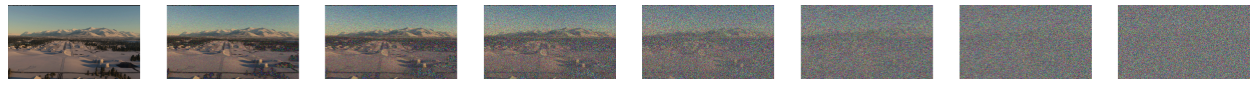
\includegraphics[width=0.8\textwidth]{figures/noise_to_image.png}
\caption{Diffusion forward process}
\label{fig:noise_to_image}
\end{figure}

The intuition of Diffusion models is that, if a model can be trained to predict the noise in an image at a *timestep*, we can start at pure noise, then repeatedly call this model and remove the noise from the image, at each step making a less noisy image.

A key architecture used in diffusion models are U-Nets, introduced in \cite{ronneberger_u-net_2015}. The U-Net is composed of two parts: an encoder and a decoder. The encoder transforms the image into a compressed form that retains essential features. This compressed data is called a "latent". The decoder can then operate on this latent and output some data related to the input data. In the original paper, they used the U-Net to extract biomedical segmentation data. In Diffusion models, the U-Net is used as the model that predicts the noise from an image.

\begin{figure}[htbp]
\centering
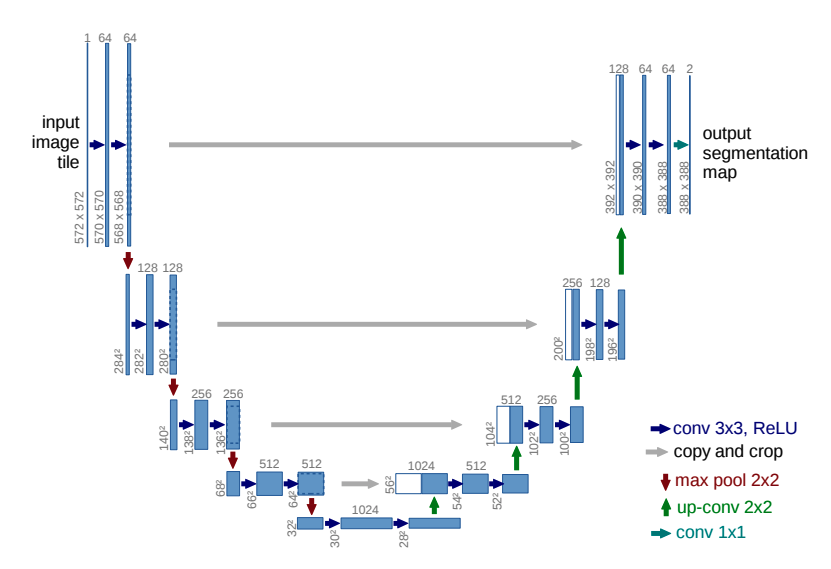
\includegraphics[width=0.8\textwidth]{figures/unet_architecture.png}
\caption{Figure from \cite{ronneberger_u-net_2015}}
\label{fig:unet_architecture}
\end{figure}

Although recently diffusion models have emerged as the new state-of-the-art architecture for image generation \cite{yang_diffusion_2024}, they do have disadvantages. Namely, their inference time is slower than of GANs, they have a higher computational cost, and by themselves, they lack mechanisms for precise editing of the image aside from the text prompt.

This problem of controlling the generated image was tackled by \cite{zhang_adding_2023}, that introduced ControlNet. ControlNet is a neural network that allows spatial conditioning to pre-trained text-to-image models. With it, it is possible to use canny edges, human poses, and segmentation masks to control the final result of the image. This allows greater control over the generation of synthetic images, such as the positioning of a runway in an image or control over the markings and detailed paintings on the runway.

\section{Synthetic datasets built with diffusion models}

In \cite{saragih_using_2024}, the authors cite a similar data scarcity problem in the field of medical images, specifically, gastrointestinal images. To solve this problem, they built a pipeline that used diffusion models to generate labeled gastrointestinal polyp images.

They started by clustering the training images and masks into 20 different clusters, and after that, training a four-channel (3 for RGB and a binary one for the mask) DDPM (Denoising Diffusion Probabilistic Models) model for each cluster. The models were trained with a fourth channel so that the model outputs an image and the associated mask along with it, requiring no human labelling. They used the RePaint \cite{lugmayr_repaint_2022} technique to guide the diffusion process so that the polyp was always generated in a specific area of the images, and they also used styling techniques so that the generated images were realistic. 

They compared the diffusion generated images with a GAN model generated images and found that the diffusion images were closer to real ones. The study trains several diffusion models to address the problem of large variation between images in the dataset, making each diffusion model "specialized" in generating images similar to its cluster. The paper shows promising results that we can augment image datasets with diffusion models, but only low resolution images were generated (256x256 pixels) and a larger variety of images would require training more independent models.

In \cite{reutov_generating_2023}, the author explored using text-to-image diffusion model to generate urban traffic images for vehicles detection and classification. The author used the trained Kandinsky 2.2 model to generate images using prompt engineering, the practice of crafting a prompt so the image contains the necessary details. 192 different prompt variants were used to generate 1000 images with different combinations of traffic density, type of vehicle, location, weather condition, time of day, and camera location. The paper shows how far off-the-shelf models are capable of generating realistic images that can be used to train detection algorithms. But, it does not compare images generated by different models and the images have to be manually labeled. 

In \cite{voetman_big_2023}, the authors studied the effectiveness of fine-tuning a pre-trained Stable Diffusion model for the purpose of generating datasets, applied to apple detection in apple orchards. They separated their baseline dataset into two datasets: green apples and red apples. After that, they fine-tuned two Stable Diffusion models with DreamBooth, and then generated a whole dataset. They used a trained apple detection model for baseline image annotations and then manually refined these annotations. To experimentally test the effectiveness of their datasets, they trained multiple YOLO object detectors on the baseline and synthetic datasets and compared the results. In their study, object detectors performed similarly when trained on their synthetic dataset and when trained on real images datasets. Their approach shows promising results in dataset generation with Stable Diffusion, although there is a lack of diversity (e.g. weather conditions, lighting conditions, different backgrounds, etc...) in both the baseline dataset that makes it easier to generate a synthetic dataset that is similar to the original.

\section{Evaluation of Synthetic Data}

Across the previously mentioned works, two types of evaluation were common: theoretical similarity and experimental performance. Theoretical similarity were done using metrics such as FID (Fréchet Inception Distance) \cite{heusel_gans_2017} and SSIM (Structural Similarity Index) \cite{wang_image_2004}, which measure the similarity between two images. Theoretical similarity was used to evaluate the synthetic datasets in \cite{saragih_using_2024}. Experimental performance, on the other hand, is about training a real model on the synthetic dataset and comparing the results. Experimental performance was used to evaluate the synthetic datasets in all runway segmentation papers covered in this review, except for LARD, and in \cite{reutov_generating_2023} and \cite{voetman_big_2023}.

Both forms of testing are valid and have their trade-offs. Theoretical similarity is faster and easier to measure, but heavily depends on what images are included in the test. And if a dataset contains very different images' structures than the original, even if they are high-quality, the FID/SSIM give worse values. On the other hand, experimental performance tests the dataset in a realistic setting, evaluating how it will be used by other researchers, but suffers from the joint dataset-model problem covered previously.

%*****************************************
%*****************************************
%*****************************************
%*****************************************
%*****************************************


\cleardoublepage
\part{Methodology and Development}\label{pt:methodology}

\chapter{Design}

\section{Project overview}

The literature review has shown the importance of large-scale, public, and diverse datasets for deep-learning projects, specifically, in the field of runway detection and segmentation, where there is currently a lack of a dataset of real images with these characteristics. To address this challenge, previous work on the field has relied on synthetic data, mainly collected from flight simulators, which poses a significant cost barrier to the expansion of these datasets as these simulators are usually paid and closed-source, and the collected images require manual labelling.

At the same time, the emergence of diffusion models as the new state-of-the-art technique in image generation has opened a new window of opportunity in building synthetic datasets. Although this idea of using diffusion models to build synthetic datasets has been explored in other fields, there is no known work applying it to the runway segmentation research field.

This project's primary research question is \emph{how can a suitable synthetic
image dataset be built for computational vision tasks without the need of images
extracted from simulators or similar solutions}. To answer this question, the project uses the field of vision-based landing and builds a synthetic runway image dataset.

The primary users of this project are researchers that may use the dataset,
\ac{GARD}, provided with this project to
build models for runway detection and segmentation. Secondary users might be
researchers interested in synthesizing their own datasets for
computational vision tasks, such as classification or segmentation, using the
\emph{Canny2Concrete} pipeline architecture, adapting it for their own needs.

With these end-users in mind, this projects delivers a two-fold contribution: a novel modular data augmentation pipeline that can increase the diversity of an existing dataset, while maintaining key features and structures; and using this data augmentation pipeline to generate a fully synthetic runway images dataset based on existing public datasets.

The proposed research question begs the question of what constitutes a "suitable synthetic image dataset". Here, we rank the following characteristics that make an image dataset suitable:

\phantomsection
\label{sec:suitable-dataset}
\begin{enumerate}
    \item \textbf{Human-judged realism}: humans subjectively judge the images as credible and realistic. When comparing side-by-side the images of the generated dataset with other datasets, the perceived quality of the images are the same or better.
    \item \textbf{Detection by existing models}: fine-tuned models on available datasets can detect the presence and segmentation of the desired data (runways in this project) in the images.
    \item \textbf{Data diversity}: the dataset has good data diversity, including edge cases and several data variations.
    \item \textbf{Model training}: an existing architecture can be trained on the dataset and achieve a reasonable performance or a pre-trained model can be fine-tuned and have their performance improved.
\end{enumerate}

\section{Data augmentation pipeline}

On earlier prototypes, several diffusion techniques such as prompt engineering, prompt weighting, unconditional image generation, inpainting and textual inversion were tried. Most of them failed to, standalone, generate realistic runway images with detailed and accurate markings. The most successful attempt was using ControlNet with an input canny edge, alongside well-crafted prompts to guide the text-to-image model. Because the canny edge was extracted from an existing runway image, the generated image faithfully respected the runway shape, position, markings and texture. Thus, the data augmentation pipeline is based around using a text-to-image diffusion model with ControlNet.

The data augmentation pipeline is composed of four separate modules, that can each be independently developed and improved, or totally replaced without affecting the overall functioning of the pipeline. This modularity and separation of concerns is good software engineering practice and aids on future research developing on this project.

\begin{description}
    \item[\textbf{Template image selection module}]: this step selects the "template images" that will be used in the pipeline. The template images are existing images in public datasets that are used to extract the overall structure of the image containing the runway to be used in the image generation step. Ideal template images have clear visibility of the runway and the surrounding background.  The output of this module is a folder with pairs of image files and label files.

    \item[\textbf{Edge extraction module}]: this step uses the template images as input, processes them, and outputs canny edge images, to be used as inputs for ControlNet, alongside the according label for that image.

    \item[\textbf{Base Image generation module}]: this step uses as inputs the canny edges, a list of text prompts, and a number of how many images should be generated for each pair of canny edge and prompt. It then uses a text-to-image model with ControlNet to generate base images.

    \item[\textbf{Variant image generation module}]: this module uses as input
      the base images and apply a series of transformations to them, such as
      applying rotations and occlusion effects to the image.
\end{description}

\begin{figure}[htbp]
\centering
\includegraphics[width=1.2\textwidth]{figures/Canny2Concrete.png}
  \caption{Diagram of the \emph{Canny2Concrete} pipeline, with real images as
  examples.}
\end{figure}

\FloatBarrier
\section{Evaluation}

Following the standards of evaluation of synthetic datasets presented in the literature review, and our definition of what constitutes a suitable synthetic dataset, two types of evaluation will be done on the dataset: intrinsic and experimental evaluation.

Intrinsic evaluation measures the quality of a dataset by its intrinsic characteristics, such as image realism, resolution, diversity, and size. Ideally, to judge human-based realism, a group of subject experts would be assembled to judge the images, but because of time-constraints, this won't be done.

Instead, it will be replaced by metrics of image similarity between template
images and the generated base images. Through metrics such as FID (Fréchet
Inception Distance) and SSIM (Structural Similarity Index) it is possible to
know how similar or different the images are from one another, and if they
retain similar structures, such as the runway shape, position, and markings, and background.

Other metrics such as size and image resolution will be reported. Data diversity will also be reported based on the generated images' text prompts. This doesn't guarantee full accuracy as there is a possibility of the model "hallucinating" and not generating a certain desired characteristic (e.g. rain, snow, runway occlusion), but nonetheless allows a good estimate to be reported.

Experimental evaluation is about using the dataset to train one or a collection of models and evaluating their performance empirically. It is an imperfect measurement, as there is a lot of moving parts when training a model, and, as seen on the literature review, a poor performance might be due to the dataset quality or an inherent flaw in the model's architecture. However, this type of evaluation is still widely used and a standard in testing synthetic datasets.

As it is not the focus of this project building a new architecture for runway
segmentation, the experimental evaluation will be restricted to training and
fine-tuning existing detection and segmentation models, such as YOLO
\cite{jocher_ultralytics_2023}.

Using a pre-trained segmentation model, comparisons will be made between the
performance of training on this new synthetic dataset and of existing datasets,
and the resulting performance when detecting a real images dataset. The main
metric used will be \ac{mAP}, at different levels of recall thresholds.

\chapter{Implementation}

% \documentclass[12pt]{article}

% \usepackage[utf8]{inputenc}
% \usepackage[T1]{fontenc}
% \usepackage{lmodern}        % For improved text clarity
% \usepackage{geometry}       % For page layout
% \usepackage{hyperref}       % For hyperlinks
% \usepackage{graphicx}       % For figures/images
% \usepackage{listings}       % For code listings
% \usepackage{amsmath,amssymb}

% % Set up the listings environment for Python

% \begin{document}

% \section{Implementation}

\section{Pipeline}

The pipeline is implemented through four Jupyter notebooks, one for each module.

\subsection{Template image selection module}

The template image selection module contains an adapter function that reads images from the public LARD dataset \cite{ducoffe_lard_2023}, generates JSON label files, and places the image-label file pairs into the output directory. 
The LARD dataset is composed of several different folders containing both synthetic and real images. 
It has two real images folders: \emph{Nominal cases} and \emph{Edge cases}, the latter being composed of images with poor runway visibility.

Because the template images are used to extract canny edges, it is better to use images with clear runway and surrounding area visibility. 
Hence, the \emph{Nominal cases} folder, containing 1500 images, was chosen.

The images are then processed into square format, since Stable Diffusion naturally works with square images. 
The runway is horizontally centered so it will not be out of frame when cropping into a square. 
The following code does this:

\begin{lstlisting}
xs = [p[0] for p in pts]
ys = [p[1] for p in pts]
min_x, max_x = min(xs), max(xs)
min_y, max_y = min(ys), max(ys)

# Vertical crop is the entire height
top = 0
bottom = H

# Horizontal positioning for H-wide crop
center_x = (min_x + max_x) / 2.0
ideal_left = int(round(center_x - (H / 2)))
left = max(0, min(ideal_left, W - H))
right = left + H

cropped_img = img.crop((left, top, right, bottom))
\end{lstlisting}

Then, the new shifted runway corners' keypoints are computed to build a JSON label:

\begin{lstlisting}
shifted_pts = [(p[0] - left, p[1] - top) for p in pts]

# Build label
image_label = ImageLabel(
    dataset="LARD/LARD_test_real_nominal",
    sourceImage=os.path.basename(image_path),
    runwayLabel=shifted_pts
)
\end{lstlisting}

Finally, the image label is converted to JSON, and both the cropped images and their labels are saved to the output folder.

\subsection{Edge extraction module}

The edge extraction module contains a generator function that takes an input directory and outputs a directory with corresponding canny edge images at a $1024 \times 1024$ resolution. 
The generator function uses an image processor from a ControlNet Auxiliary library to generate the canny edges, and then resizes to the desired resolution:

\begin{lstlisting}
from controlnet_aux.processor import Processor

processor = Processor(
    'canny',
    {
        "detect_resolution": 756,
        "image_resolution": 1024
    }
)

pil_in = Image.open(image_path).convert("RGB")
canny_pil = processor(pil_in, to_pil=True).resize((1024, 1024))
\end{lstlisting}

To help in the image generation process, a polygon is drawn onto the image to delimit the area of the runway:

\begin{lstlisting}
cv2.polylines(
    canny_array,
    [corners_sorted.astype(np.int32)],
    isClosed=True,
    color=(255, 255, 255),
    thickness=2
)
\end{lstlisting}

Finally, the corners are scaled to this new image resolution and saved to the new label file:

\begin{lstlisting}
orig_h, orig_w = image_bgr.shape[:2]
corners_array = np.array(runway_corners, dtype=np.float32)
corners_array[:, 0] *= (1024.0 / orig_w)
corners_array[:, 1] *= (1024.0 / orig_h)
\end{lstlisting}

\subsection{Base Image generation module}

This is the most important module of the pipeline, as everything depends on the quality of the base images generated in this step. 
To generate the images, the \texttt{diffusers} library \cite{???} is used, providing utilities for generating images with diffusion models.

The classes one needs from \texttt{diffusers} depend on which model is in use. 
The DreamShaper model \cite{???} is a general-purpose Stable Diffusion model, meant to compete with other general-purpose models such as DALL-E and Midjourney. 
Of several tested models and pipelines, DreamShaper was chosen for its image quality, faithfulness to the prompt, and ability to construct diverse scenarios (ranging across different lighting and weather conditions).

From the DreamShaper family, we chose the DreamShaper XL version, capable of producing $1024 \times 1024$ images, as it is based on Stable Diffusion XL. 
This higher resolution was necessary to generate finer details such as runway markings.

Having selected DreamShaper XL, the rest follows naturally. 
For the ControlNet model, the pre-trained canny-edge-based ControlNet offered by \texttt{diffusers} for Stable Diffusion XL was used, and the recommended scheduler configuration for DreamShaper was applied:

\begin{lstlisting}
controlnet = ControlNetModel.from_pretrained(
    "diffusers/controlnet-canny-sdxl-1.0", torch_dtype=torch.float16
)

pipeline = StableDiffusionXLControlNetPipeline.from_pretrained(
    "lykon/dreamshaper-xl-v2-turbo",
    torch_dtype=torch.float16,
    variant="fp16",
    controlnet=controlnet
).to("cuda")

pipeline.scheduler = DPMSolverMultistepScheduler.from_config(
    pipeline.scheduler.config,
    algorithm_type="sde-dpmsolver++",
    use_karras_sigmas=True
)

pipeline.enable_model_cpu_offload()
\end{lstlisting}

A critical part of generative models is \emph{prompt engineering}: crafting an input prompt that achieves the desired result. 
Diffusion models accept both a \emph{prompt} and a \emph{negative prompt}. 
The model tries to produce what is mentioned in the prompt and avoid what is mentioned in the negative prompt.

Crafting the prompt is a process of trial and error until satisfactory results are found. 
In practice, it is helpful to look at prompts used in the model's example pages to see keywords the model responds strongly to, such as \texttt{cinematic film still}, \texttt{realistic}, \texttt{ugly}, or \texttt{deformed}.

Since this project needed to create images under diverse scenarios, two base prompts were defined for daylight images with no weather adversity, and a dictionary of modifiers was used to add or remove keywords to achieve weather or time-of-day effects:

\begin{lstlisting}
base_prompt = "photo of airport runway, aerial view, 4k, cinematic film still, realistic, beautiful landscape around, high-contrast runway lines"

base_neg = "airplane, ugly, low-quality, ugly background, ugly airstrip, deformed, dark, noisy, blurry, low contrast, missing lines, unrealistic, drawing, objects on runway"

modifiers = {
    "rain": (
        "+raining +storm +wet",
        "-dark -noisy -blurry",
    ),
    "fog": (
        "+(harsh fog) +mist +haze",
        "-dark -noisy -blurry",
    ),
    "snow": (
        "+snowing",
        "",
    ),
    "dusk": (
        "+(at dusk)",
        "",
    ),
    "dawn": (
        "+(at dawn)",
        "",
    ),
    "night": (
        "+(at night)",
        "-dark",
    )
}
\end{lstlisting}

A helper function (e.g., \texttt{apply\_modifiers}) builds the final prompts (and negative prompts) from the base prompts and these modifiers. 
It also receives the number of images to generate, returning a data structure that can be passed to \texttt{generate\_base\_images}, which uses the prompt pairs to generate and save images:

\begin{lstlisting}
generate_base_images(
    "p_FilteredCannyEdges",  # input directory
    "p_BaseImages",          # output directory
    prompt_pairs=[           # images to generate
        apply_modifiers("day", [], 5),
        apply_modifiers("night", ["night"], 5),
        apply_modifiers("dusk", ["dusk"], 1),
        apply_modifiers("dawn", ["dawn"], 1),
        apply_modifiers("fog", ["fog"], 1),
        apply_modifiers("fog+night", ["night", "fog"], 1),
        apply_modifiers("rain", ["rain"], 1),
        apply_modifiers("rain+night", ["night", "rain"], 1),
        apply_modifiers("snow", ["snow"], 1),
        apply_modifiers("snow+night", ["night", "snow"], 1),
    ],
    model_name="sdxl-dreamshaperxl",
    # show=True
)
\end{lstlisting}

\subsection{Variant image generation module}

To generate variant images, three pipelines are run: a positional variant augmentation, outpainting the borders, and weather occlusion effects.

The first pipeline uses the \emph{Albumentations} library \cite{???} to run three transformations: 
(1) random horizontal flip, 
(2) padding with a border (to simulate a more distant runway), and 
(3) slight random rotation from $-25^\circ$ to $+25^\circ$:

\begin{lstlisting}
pipeline = A.ReplayCompose(
    [
        A.HorizontalFlip(p=0.5),
        A.CropAndPad(
            px=((51, 410),  # top
                (51, 410),  # bottom
                (51, 410),  # left
                (51, 410)), # right
            keep_size=False,
            p=1.0
        ),
        A.Affine(rotate=(-25, 25), p=1.0),
    ],
    keypoint_params=A.KeypointParams(format='xy', remove_invisible=False)
)
\end{lstlisting}

\begin{figure}[htbp]
\centering
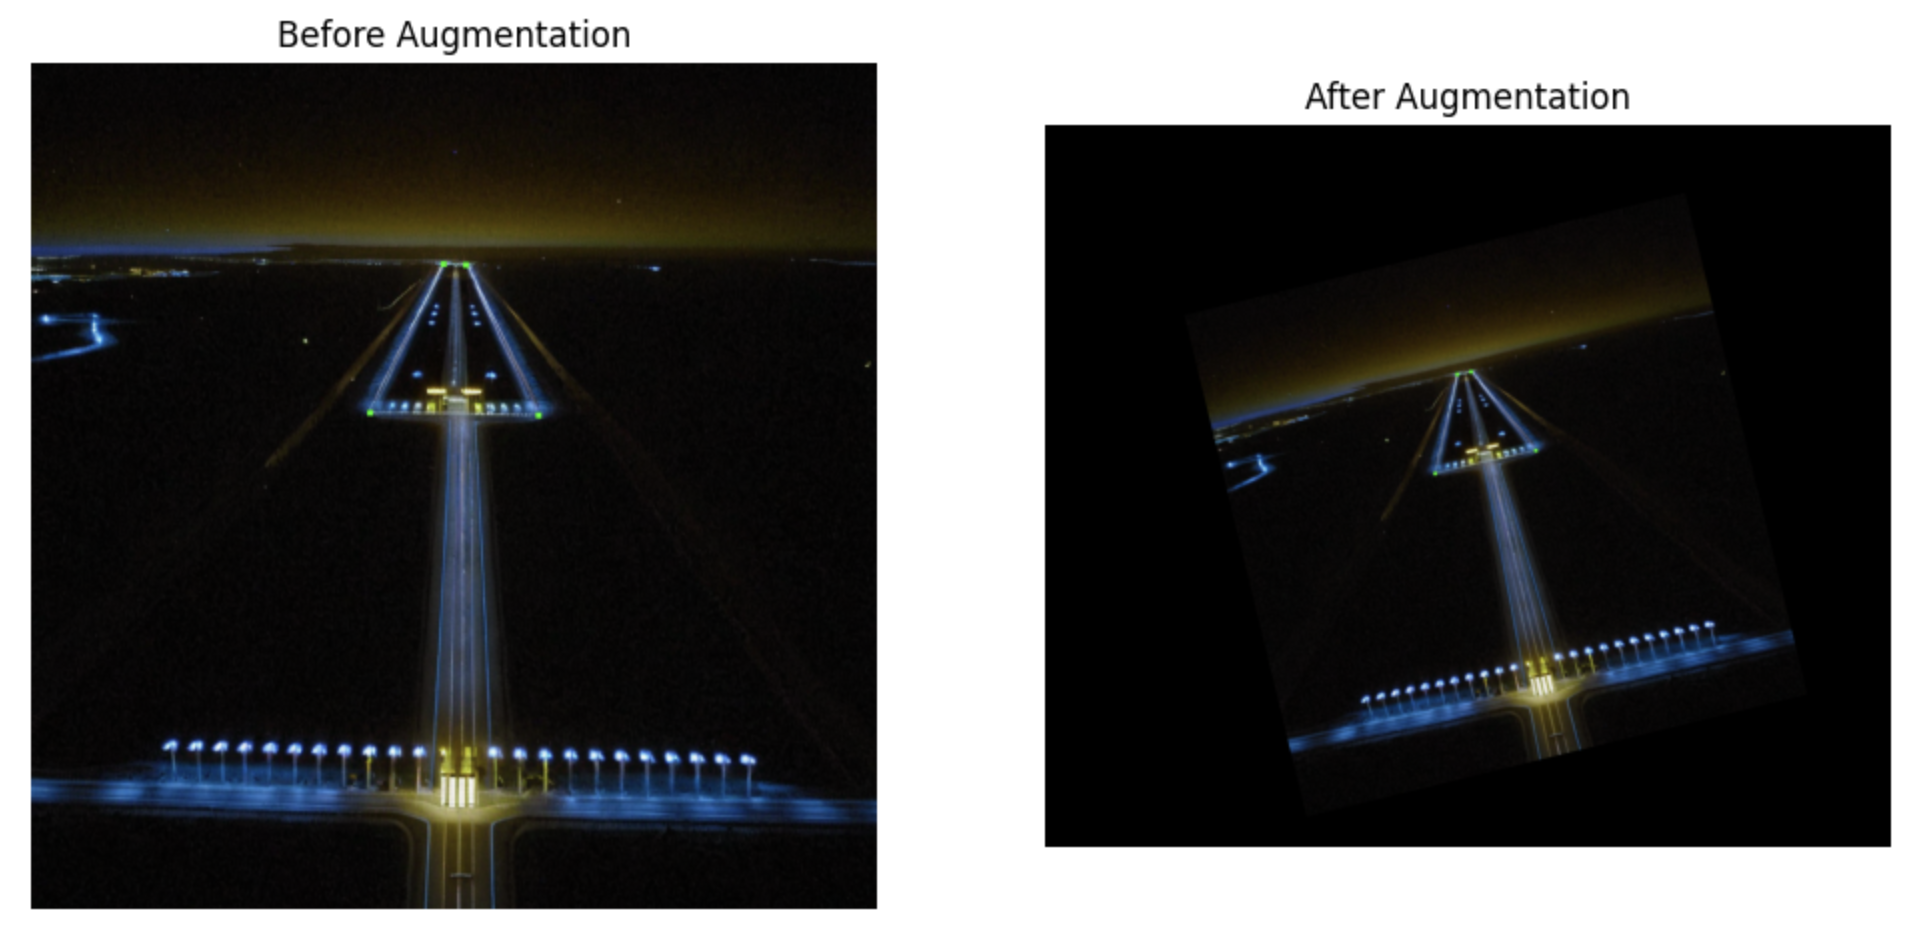
\includegraphics[width=1.0\textwidth]{figures/albumentations.png}
  \caption{Applying the \emph{Albumentations} pipeline to an image.}
\label{fig:noise_to_image}
\end{figure}

This pipeline generates images with black borders. 
The second pipeline uses \emph{inpainting} to fill in these black borders. 
First, OpenCV-based inpainting is used, filling the black border with colors from the nearby region. 
Then, a Stable Diffusion model refines the borders for better blending.

OpenCV implements Alexandru Telea's inpainting algorithm [TODO: ADD CITATION TO
TELEA] via \texttt{cv2.inpaint} with the \texttt{cv2.INPAINT\_TELEA} flag:

\begin{lstlisting}
mask = np.all(image == 0, axis=2).astype(np.uint8) * 255
kernel = np.ones((3, 3), np.uint8)
mask = cv2.dilate(mask, kernel, iterations=4)
image = Image.fromarray(cv2.cvtColor(
    cv2.inpaint(image, mask, 3, cv2.INPAINT_TELEA),
    cv2.COLOR_BGR2RGB
))
\end{lstlisting}

After this initial inpainting, a Stable Diffusion XL Inpainting pipeline is used to process the image. 
The original prompts used for the base images are reused, along with a blurred mask for smoother blending:

\begin{lstlisting}
pipe = StableDiffusionXLInpaintPipeline.from_pretrained(
    "lykon/dreamshaper-xl-lightning",
    torch_dtype=torch.float16,
    variant="fp16",
).to("cuda")
pipe.scheduler = DPMSolverMultistepScheduler.from_config(pipe.scheduler.config)

# [...]

mask = pipe.mask_processor.blur(Image.fromarray(mask), blur_factor=75)

result = pipe(
    prompt=data["prompt"],
    negative_prompt=data["negative_prompt"],
    image=image,
    mask_image=mask,
    strength=0.8,
    generator=generator,
    num_inference_steps=30,
    guidance_scale=2,
).images[0]
\end{lstlisting}

The third pipeline reads the images output by the second pipeline and creates a new folder with the same images, further augmented with weather occlusion effects done by \texttt{imgaug} \cite{???}. 
Effects are chosen depending on the variant:

\begin{itemize}
\item Clouds for \emph{pure} \texttt{day/night/dusk/dawn} images
\item Fog for \texttt{fog} images
\item Rain for \texttt{rain} images
\item Snowflakes for \texttt{snow} images
\end{itemize}

For example:

\begin{lstlisting}
if variant in ["day", "night", "dusk", "dawn"]:
    aug = iaa.SomeOf((1, 2), [
        iaa.CloudLayer(...),
        iaa.CloudLayer(...),
    ])
    image = aug(image=image)
    applied_effects.append("clouds")
elif variant in ["fog", "fog+night"]:
    aug = iaa.CloudLayer(...)
    image = aug(image=image)
    applied_effects.append("fog")
elif variant in ["rain", "rain+night"]:
    aug = iaa.Rain(drop_size=(0.1, 0.2), speed=(0.01, 0.05))
    image = aug(image=image)
    applied_effects.append("light_rain")
elif variant in ["snow", "snow+night"]:
    aug = iaa.Snowflakes(flake_size=(0.1, 0.3), speed=(0.01, 0.05))
    image = aug(image=image)
    applied_effects.append("snowflakes")
\end{lstlisting}

After each augmentation pipeline, the label JSON file is enriched with data to ensure reproducibility, including random seeds and applied transformations.

\section{Filtering Tool}

A manual filtering tool was implemented in Python with OpenCV to assist in selecting template images. 
It reads images from a directory and allows pressing \texttt{Space} to select an image or \texttt{X} to discard. 
Selected images are copied into a new directory, and a log file retains progress so the tool can be closed and resumed later without starting from scratch.

Due to time constraints, template images were filtered as follows:
\begin{enumerate}
\item Use all images from \texttt{LARD\_test\_real\_nominal} as template images, pass them through the canny-edge and base-image generation modules, generating one daylight base image per template.
\item Use the filtering tool to select which base images had easily recognizable runways with consistent markings and structure.
\item In the end, 361 images were selected, and only these canny edges were used to generate all images in the final dataset.
\end{enumerate}

\section{The final datasets}

Three datasets are published:

\begin{enumerate}
\item \texttt{BaseImages}: containing 6498 images (18 variations for each of the 361 canny edge images).
\item \texttt{VariantImages}: containing 19494 images (3 variations for each base image) \emph{before} weather occlusion.
\item \texttt{VariantImagesWithOcclusion}: also 19494 images, same as \texttt{VariantImages} but with weather effects applied.
\end{enumerate}

Each image is associated with four files:
\begin{enumerate}
\item \texttt{.png} file (the image itself).
\item \texttt{.json} file (the image label).
\item \texttt{.mask.png} file (a segmentation mask: black background, white runway).
\item \texttt{.txt} file (a YOLO-format label for detection/segmentation training).
\end{enumerate}

The JSON label file carries the runway keypoints as well as all data required for reproducing that specific image, including prompts, seeds, variant details, transformations, and so on. 
This metadata supports image classification (by variant or weather type), label fixes without regenerating images, and easier reproducibility/peer review.

Each directory also includes \texttt{train.txt}, \texttt{test.txt}, and \texttt{val.txt} splits in 80/10/10 proportions, ensuring images sharing the same source canny edge (and thus similar structure) do not leak from training into testing.

\section{Generated images}


To demonstrate a sample of generated images, three random template images were
chosen. Two are close-up shots and the third is a far away picture. They
are shown as three grids of images of for rows.

The first row contains the template image, the canny edge extracted from it,
and the runway label mask. The second row contains three images from the Base
Images dataset generated from the template image. The third row contains three
images from the Variant Images dataset, generated from the Base Images. The
fourth row contains three images from the Variant Images with Occlusion dataset,
associated with the shown Variant Images.

\begin{figure}[htbp]
\centering
\includegraphics[width=1.2\textwidth]{figures/GeneratedImage1.png}
  \caption{Template image \emph{"9xG0a8TUdXg\_028"} }
\label{fig:noise_to_image}
\end{figure}

\begin{figure}[htbp]
\centering
\includegraphics[width=1.2\textwidth]{figures/GeneratedImage2.png}
  \caption{Template image \emph{"0CLSYZPFbTg\_110"} }
\label{fig:noise_to_image}
\end{figure}

\begin{figure}[htbp]
\centering
\includegraphics[width=1.2\textwidth]{figures/GeneratedImage3.png}
  \caption{Template image \emph{"0P-HJgLkZLk\_085"} }
\label{fig:noise_to_image}
\end{figure}


\cleardoublepage
\part{Results and Discussion}\label{pt:results}
\chapter{Evaluation}

\section{Generated Datasets}

After filtering the template images manually using the Filtering Tool and
the methodology described in Chapter 4, a total of 361 template images were
selected.

Using the Canny2Concrete pipeline with these filtered template images,
\emph{GARD} was generated, containing a total of 45486 images, separated
into three datasets:

\begin{enumerate}
\item \texttt{BaseImages}: containing 6498 images (18 variations for each of the 361 canny edge images).
\item \texttt{VariantImages}: containing 19494 images (3 variations for each base image) \emph{before} weather occlusion.
\item \texttt{VariantImagesWithOcclusion}: also 19494 images, same as \texttt{VariantImages} but with weather effects applied.
\end{enumerate}

\section{Sample Images}

To demonstrate a sample of generated images, three random template images were
chosen. Two are close-up shots and the third is a far away picture. They
are shown as three grids of images of for rows.

The first row contains the template image, the canny edge extracted from it,
and the runway label mask. The second row contains three images from the Base
Images dataset generated from the template image. The third row contains three
images from the Variant Images dataset, generated from the Base Images. The
fourth row contains three images from the Variant Images with Occlusion dataset,
associated with the shown Variant Images.

\begin{figure}[htbp]
\centering
\includegraphics[width=1.2\textwidth]{figures/GeneratedImage1.png}
  \caption{Images generated from the template image \emph{"9xG0a8TUdXg\_028"} }
\label{fig:noise_to_image}
\end{figure}

\begin{figure}[htbp]
\centering
\includegraphics[width=1.2\textwidth]{figures/GeneratedImage2.png}
  \caption{Images generated from the template image \emph{"0CLSYZPFbTg\_110"} }
\label{fig:noise_to_image}
\end{figure}

\begin{figure}[htbp]
\centering
\includegraphics[width=1.2\textwidth]{figures/GeneratedImage3.png}
  \caption{Images generated from the template image \emph{"0P-HJgLkZLk\_085"} }
\label{fig:noise_to_image}
\end{figure}

\FloatBarrier
\section{Intrinsic Evaluation}

The chosen metric for intrinsic evaluation was SSIM (Structural Similarity Index Measure) \cite{wang_image_2004}. 
SSIM evaluates how similar two images are to each other. 
An SSIM of 1 indicates perfect similarity (i.e., the image compared with itself), a score of 0 indicates no similarity, and a score of -1 represents perfect anti-correlation.

It is difficult to define what constitutes a good SSIM value. 
For example, a realistic and high-quality background that significantly differs from the original image would reduce the SSIM score, despite not being inherently negative. 
On the other hand, since the generated image is based on the canny edge structure of the template image, we should expect a positive correlation if the generation process is functioning as intended.

\begin{figure}[htbp]
% \centering
\hspace*{-2.5cm} % shift left by 1.5 centimeters
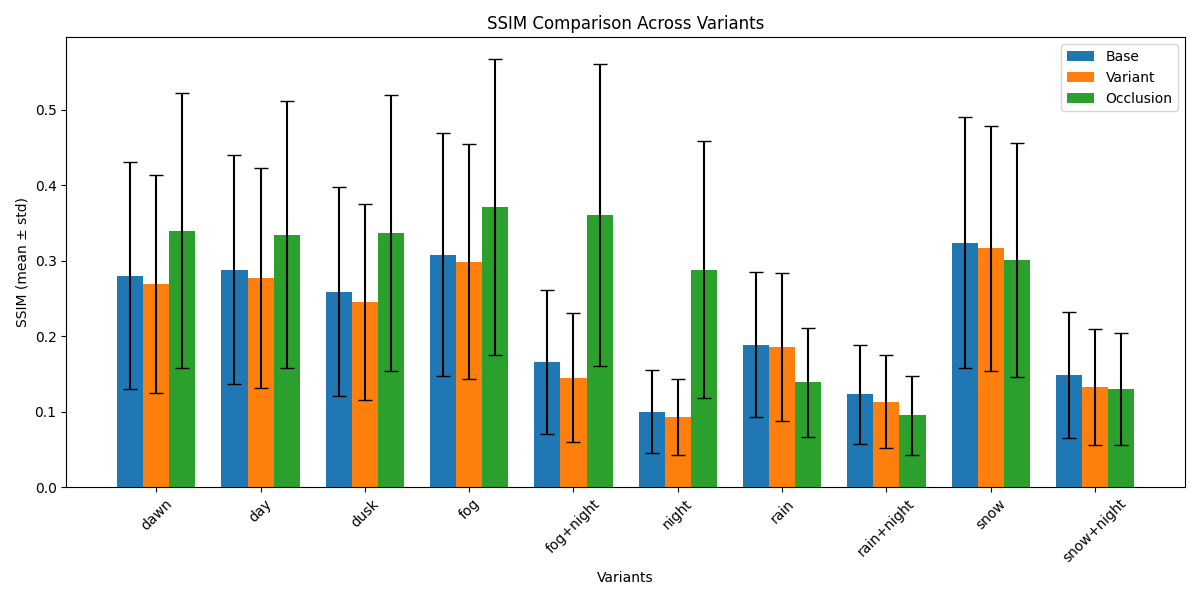
\includegraphics[width=1.5\textwidth]{figures/SSIM.png}
  \caption{SSIM Comparison Across Variants and Datasets}
\label{fig:noise_to_image}
\end{figure}

These are positive results, clearly indicating that the data augmentation process is functioning as expected. 
The generated images are positively correlated with the template images---as expected in a data augmentation pipeline---while the similarity significantly drops as diversity is introduced.

\FloatBarrier
\section{Experimental Evaluation}

Following the methodology of \cite{voetman_big_2023}, for extrinsic evaluation, several pre-trained segmentation models are fine-tuned, comparing their performance when trained exclusively on the synthetic images of LARD \cite{ducoffe_lard_2023} and when trained on the project's datasets.

To validate the performance of the trained models, the human-labeled real images of the LARD dataset are used. The real images in LARD are divided into two folders: \emph{nominal cases} and \emph{edge cases}, the latter containing images with poor runway visibility.

Three pre-trained models from the YOLO v11 family are fine-tuned: YOLO11n (``n'' for nano), YOLO11s (``s'' for small), and YOLO11m (``m'' for medium). The larger models YOLO11l and YOLO11x were not trained due to hardware constraints.

YOLO reports metrics for two tasks: detection (bounding box evaluation) and
segmentation (segmentation mask evaluation). The metric used to compare the
performance is mAP (mean Average Precision), which is the average of the
precision-recall curve. The mAP is calculated at three different IoU (Intersection over Union) thresholds: 50\%, 75\%, and 50:95.

Two tables (Tables~\ref{tab:nominal_results} and~\ref{tab:edge_cases_results}) are presented, one for the nominal dataset and another for the edge
cases dataset. The tables show the performance of the models when trained on the
LARD dataset and the GARD datasets, with the differences in performance
highlighted, with a positive value indicating an improvement in performance of
the model trained on the GARD dataset over the comparable one with the LARD dataset.

Based on the experimental evaluation metrics, the results are overwhelmingly
positive, as the GARD dataset has consistently 
matched or outperformed the LARD dataset in most cases. Especially in the
Edge Cases dataset, which is the most challenging, the GARD dataset shows
outpeformance across all models, tasks (detection and segmentation), and mAP
thresholds.

\medskip

\begin{table}[htbp]
\centering
\small
\setlength{\tabcolsep}{4pt}
\renewcommand{\arraystretch}{1.2}

  \caption{Validation with real images from LARD dataset, \emph{Nominal} dataset: YOLO11n/s/m performance comparison between LARD and GARD variants, with per-variant differences ($\Delta$).}
  \label{tab:nominal_results}

\begin{tabular}{|c|c|ccc|ccc|}
\hline
\multirow{2}{*}{\textbf{Model}} &
\multirow{2}{*}{\textbf{Dataset}} &
\multicolumn{3}{c|}{\textbf{Detection (mAP)}} &
\multicolumn{3}{c|}{\textbf{Segmentation (mAP)}} \\
& & @50:95 & @50 & @75 & @50:95 & @50 & @75 \\

\hline
\multirow{6}{*}{YOLO11n}
& Baseline (LARD) & 0.691 & 0.862 & 0.790 & 0.485 & 0.833 & 0.507 \\
& GARD BaseImages & 0.722 & 0.874 & 0.796 & 0.452 & 0.828 & 0.441 \\
& $\Delta$ & \textbf{+0.031} & \textbf{+0.012} & \textbf{+0.006} & \textbf{-0.033} & \textbf{-0.005} & \textbf{-0.066} \\
& GARD VariantImages & 0.735 & 0.888 & 0.807 & 0.471 & 0.842 & 0.472 \\
& $\Delta$ & \textbf{+0.044} & \textbf{+0.026} & \textbf{+0.017} & \textbf{-0.014} & \textbf{+0.009} & \textbf{-0.035} \\
& GARD VariantWithOcclusion & 0.728 & 0.899 & 0.794 & 0.469 & 0.841 & 0.467 \\
& $\Delta$ & \textbf{+0.037} & \textbf{+0.037} & \textbf{+0.004} & \textbf{-0.016} & \textbf{+0.008} & \textbf{-0.040} \\
\hline

\hline
\multirow{6}{*}{YOLO11s}
& Baseline (LARD) & 0.709 & 0.870 & 0.807 & 0.498 & 0.842 & 0.526 \\
& GARD BaseImages & 0.747 & 0.894 & 0.819 & 0.454 & 0.843 & 0.432 \\
& $\Delta$ & \textbf{+0.038} & \textbf{+0.024} & \textbf{+0.012} & \textbf{-0.044} & \textbf{+0.001} & \textbf{-0.094} \\
& GARD VariantImages & 0.780 & 0.915 & 0.846 & 0.485 & 0.873 & 0.482 \\
& $\Delta$ & \textbf{+0.071} & \textbf{+0.045} & \textbf{+0.039} & \textbf{-0.013} & \textbf{+0.031} & \textbf{-0.044} \\
& GARD VariantWithOcclusion & 0.771 & 0.914 & 0.845 & 0.481 & 0.870 & 0.476 \\
& $\Delta$ & \textbf{+0.062} & \textbf{+0.044} & \textbf{+0.038} & \textbf{-0.017} & \textbf{+0.028} & \textbf{-0.050} \\
\hline


\hline
\multirow{6}{*}{YOLO11m}
& Baseline (LARD) & 0.742 & 0.906 & 0.841 & 0.512 & 0.870 & 0.529 \\
& GARD BaseImages & 0.747 & 0.889 & 0.825 & 0.452 & 0.836 & 0.434 \\
& $\Delta$ & \textbf{+0.005} & \textbf{-0.017} & \textbf{-0.016} & \textbf{-0.060} & \textbf{-0.034} & \textbf{-0.095} \\
& GARD VariantImages & 0.792 & 0.923 & 0.854 & 0.489 & 0.874 & 0.490 \\
& $\Delta$ & \textbf{+0.050} & \textbf{+0.017} & \textbf{+0.013} & \textbf{-0.023} & \textbf{+0.004} & \textbf{-0.039} \\
& GARD VariantWithOcclusion & 0.789 & 0.922 & 0.860 & 0.485 & 0.878 & 0.481 \\
& $\Delta$ & \textbf{+0.047} & \textbf{+0.016} & \textbf{+0.019} & \textbf{-0.027} & \textbf{+0.008} & \textbf{-0.048} \\
\hline

\end{tabular}
\end{table}


\begin{table}[htbp]
\centering
\small
\setlength{\tabcolsep}{4pt}
\renewcommand{\arraystretch}{1.2}
  \caption{Validation with real images from LARD dataset, \emph{Edge cases} dataset: YOLO11n/s/m performance comparison between LARD and GARD variants, with per-variant differences ($\Delta$).}
  \label{tab:edge_cases_results}

\begin{tabular}{|c|c|ccc|ccc|}
\hline
\multirow{2}{*}{\textbf{Model}} &
\multirow{2}{*}{\textbf{Dataset}} &
\multicolumn{3}{c|}{\textbf{Detection (mAP)}} &
\multicolumn{3}{c|}{\textbf{Segmentation (mAP)}} \\
& & @50:95 & @50 & @75 & @50:95 & @50 & @75 \\

\hline
\multirow{6}{*}{YOLO11n}
& Baseline (LARD) & 0.543 & 0.708 & 0.634 & 0.399 & 0.700 & 0.414 \\
& GARD BaseImages & 0.608 & 0.802 & 0.663 & 0.425 & 0.762 & 0.439 \\
& $\Delta$ & \textbf{+0.065} & \textbf{+0.094} & \textbf{+0.029} & \textbf{+0.026} & \textbf{+0.062} & \textbf{+0.025} \\
& GARD VariantImages & 0.627 & 0.819 & 0.702 & 0.452 & 0.786 & 0.476 \\
& $\Delta$ & \textbf{+0.084} & \textbf{+0.111} & \textbf{+0.068} & \textbf{+0.053} & \textbf{+0.086} & \textbf{+0.062} \\
& GARD VariantWithOcclusion & 0.633 & 0.850 & 0.702 & 0.456 & 0.805 & 0.465 \\
& $\Delta$ & \textbf{+0.090} & \textbf{+0.142} & \textbf{+0.068} & \textbf{+0.057} & \textbf{+0.105} & \textbf{+0.051} \\
\hline

\hline
\multirow{6}{*}{YOLO11s}
& Baseline (LARD) & 0.530 & 0.696 & 0.620 & 0.395 & 0.680 & 0.388 \\
& GARD BaseImages & 0.638 & 0.834 & 0.689 & 0.440 & 0.795 & 0.446 \\
& $\Delta$ & \textbf{+0.108} & \textbf{+0.138} & \textbf{+0.069} & \textbf{+0.045} & \textbf{+0.115} & \textbf{+0.058} \\
& GARD VariantImages & 0.686 & 0.859 & 0.772 & 0.476 & 0.827 & 0.490 \\
& $\Delta$ & \textbf{+0.156} & \textbf{+0.163} & \textbf{+0.152} & \textbf{+0.081} & \textbf{+0.147} & \textbf{+0.102} \\
& GARD VariantWithOcclusion & 0.681 & 0.883 & 0.735 & 0.470 & 0.830 & 0.478 \\
& $\Delta$ & \textbf{+0.151} & \textbf{+0.187} & \textbf{+0.115} & \textbf{+0.075} & \textbf{+0.150} & \textbf{+0.090} \\
\hline

\hline
\multirow{6}{*}{YOLO11m}
& Baseline (LARD) & 0.551 & 0.730 & 0.653 & 0.406 & 0.719 & 0.396 \\
& GARD BaseImages & 0.641 & 0.826 & 0.702 & 0.433 & 0.791 & 0.429 \\
& $\Delta$ & \textbf{+0.090} & \textbf{+0.096} & \textbf{+0.049} & \textbf{+0.027} & \textbf{+0.072} & \textbf{+0.033} \\
& GARD VariantImages & 0.684 & 0.863 & 0.747 & 0.477 & 0.813 & 0.494 \\
& $\Delta$ & \textbf{+0.133} & \textbf{+0.133} & \textbf{+0.094} & \textbf{+0.071} & \textbf{+0.094} & \textbf{+0.098} \\
& GARD VariantWithOcclusion & 0.700 & 0.887 & 0.770 & 0.484 & 0.842 & 0.492 \\
& $\Delta$ & \textbf{+0.149} & \textbf{+0.157} & \textbf{+0.117} & \textbf{+0.078} & \textbf{+0.123} & \textbf{+0.096} \\
\hline

\end{tabular}
\end{table}

\FloatBarrier
\section{Discussion}

One concern with validating trained models with the Nominal dataset is that
images from this same dataset were used as template images for the data
augmentation pipeline. This might have introduced a bias in the evaluation, as
the generated images are based on the same structure as the template images.
But, we can be confident that either there is no bias or that the bias is
minimal, as the SSIM results show positive, but small correlation score between
the template images and the generated images. Another reason why this should not
be a concern is that the fine-tuned models performed better in the Edge Cases dataset, of which no images were used in the data augmentation pipeline.

Another limitation of the experimental evaluation setup was that the models were
fine-tuned on each isolated GARD dataset, without mixing them. This might have
limited the performance of the models, as each dataset has distinct features
that could have increased the diversity of a mixed dataset.

The better performance of the LARD-based models in the Nominal dataset might be
explained by the fact that the LARD dataset contains low diversity of weather
and lighting conditions, and runway occlusion, which matches the characteristics
of the Nominal dataset. This highlights the \emph{joint hypothesis problem} that
was presented in the literature review section.

This is also corroborated by the better performance of the GARD-based models in
the Edge Cases dataset, where the better diversity and realism of the GARD
datasets allowed the models to generalize better to the unseen data.

Because of time and hardware constraints, the evaluation was limited to the
YOLO11 family of models. Future work could include more models, and more
complex pipelines dedicated for runway segmentation, such as VALNet
\cite{wang_valnet_2024}.

These results are promising, showing that the Canny2Concrete pipeline is
effective in generating realistic runway images that can be used to train
detection and segmentation models, and that the GARD datasets is a viable
alternative to existing synthetic datasets.

The biggest limitation in the Cany2Concrete pipeline is the need for template
images. This limits the variety of structures that can be generated, and require
a manual selection of images. Future work could be done in either
programatically generating canny edge images without extracting them from any
given image. It would also help if the diffusion model understood better the
concept of a aerial view of a runway, so that it wouldn't need detailed canny
edges to generate a realistic image.

Another limitation is that, due to the chosen Stable Diffusion model, the
images don't look as real photos, but more like digital art. Future work could
shrink "Sim2Real" gap. This could be done by using a different diffusion model,
or by adding another module to the pipeline that would convert images to this
more realistic style.

The pipeline could also generate better results by improving the outpainting
techniques used in the variant image generation module. The current techniques
generate noticeable borders between the original image and the outpainted
background.




\cleardoublepage
\part{Conclusion}\label{pt:conclusion}
\chapter{Conclusion}

To address the challenges of data scarcity in the field of runway detection and segmentation,
this paper introduced a novel, open-source, data augmentation technique based on a multi-step
Stable Diffusion pipeline, called Canny2Concrete.

Canny2Concrete extracts features from existing datasets and outputs images
that retain a similar structure, especially the runway shape, position, and markings, but are
customizable in respect to scenery, weather, and lighting conditions, guided by
a text prompts. The images generated by the pipeline are already
labeled, saving hours of handcraft labelling.

The pipeline is tested by augmenting real runway images from the LARD \cite{ducoffe_lard_2023}
dataset. Three datasets are generated, the Base Images dataset,
containing 6498 images, the Variant Images dataset, containing 19494 images, and
the Variant Images With Occlusion dataset, containing 19494 images. In total,
45486 images, with a diverse range of weather, lighting, background, and runway
occlusion conditions and effects were generated and are publicly on Kaggle.

All the images have along with
them a JSON file
with metadata allowing any researcher to replicate that exact image, TXT label
ready to be used in training YOLO models, and a simple binary segmentation mask
image. To the best of my knowledge, this is the largest synthetic runway
dataset publicly available.

Experimental evaluation was done training state-of-the-art detection and
segmentation models with both the new datasets and a benchmark dataset, and
these models were evaluated on a real-world dataset. The results demonstrate
the effectiveness of the Canny2Concrete pipeline in generating realistic runway
images, and the viability of diffusion-based augmentation for runway segmentation
tasks.

\section{Further Work}

The biggest limitation in the Cany2Concrete pipeline is the need for template
images. This limits the variety of structures that can be generated, and require
a manual selection of images. Future work could be done in either
programatically generating canny edge images without extracting them from any
given image. It would also help if the diffusion model understood better the
concept of a aerial view of a runway, so that it wouldn't need detailed canny
edges to generate a realistic image.

Another limitation is that, due to the chosen Stable Diffusion model, the
images don't look as real photos, but more like digital art. Future work could
shrink "Sim2Real" gap. This could be done by using a different diffusion model,
or by adding another module to the pipeline that would convert images to this
more realistic style.

The pipeline could also generate better results by improving the outpainting
techniques used in the variant image generation module. The current techniques
generate noticeable borders between the original image and the outpainted
background.




% ********************************************************************
% Backmatter
%*******************************************************
\appendix
%\renewcommand{\thechapter}{\alph{chapter}}
\cleardoublepage
\part{Appendix}
%********************************************************************
% Appendix
%*******************************************************
% If problems with the headers: get headings in appendix etc. right
%\markboth{\spacedlowsmallcaps{Appendix}}{\spacedlowsmallcaps{Appendix}}
\chapter{Appendix Test}
Lorem ipsum at nusquam appellantur his, ut eos erant homero
concludaturque. Albucius appellantur deterruisset id eam, vivendum
partiendo dissentiet ei ius. Vis melius facilisis ea, sea id convenire
referrentur, takimata adolescens ex duo. Ei harum argumentum per. Eam
vidit exerci appetere ad, ut vel zzril intellegam interpretaris.
\graffito{More dummy text.}

%Errem omnium ea per, pro congue populo ornatus cu, ex qui dicant
%nemore melius. No pri diam iriure euismod. Graecis eleifend
%appellantur quo id. Id corpora inimicus nam, facer nonummy ne pro,
%kasd repudiandae ei mei. Mea menandri mediocrem dissentiet cu, ex
%nominati imperdiet nec, sea odio duis vocent ei. Tempor everti
%appareat cu ius, ridens audiam an qui, aliquid admodum conceptam ne
%qui. Vis ea melius nostrum, mel alienum euripidis eu.

\section{Appendix Section Test}
Test: \autoref{tab:moreexample} (This reference should have a
lowercase, small caps \spacedlowsmallcaps{A} if the option
\texttt{floatperchapter} is activated, just as in the table itself
 $\rightarrow$ however, this does not work at the moment.)

\begin{table}[h]
    \myfloatalign
    \begin{tabularx}{\textwidth}{Xll} \toprule
        \tableheadline{labitur bonorum pri no} & \tableheadline{que vista}
        & \tableheadline{human} \\ \midrule
        fastidii ea ius & germano &  demonstratea \\
        suscipit instructior & titulo & personas \\
        %postulant quo & westeuropee & sanctificatec \\
        \midrule
        quaestio philosophia & facto & demonstrated \\
        %autem vulputate ex & parola & romanic \\
        %usu mucius iisque & studio & sanctificatef \\
        \bottomrule
    \end{tabularx}
    \caption[Autem usu id]{Autem usu id.}
    \label{tab:moreexample}
\end{table}

%Nulla fastidii ea ius, exerci suscipit instructior te nam, in ullum
%postulant quo. Congue quaestio philosophia his at, sea odio autem
%vulputate ex. Cu usu mucius iisque voluptua. Sit maiorum propriae at,
%ea cum primis intellegat. Hinc cotidieque reprehendunt eu nec. Autem
%timeam deleniti usu id, in nec nibh altera.




\section{Another Appendix Section Test}
Equidem detraxit cu nam, vix eu delenit periculis. Eos ut vero
constituto, no vidit propriae complectitur sea. Diceret nonummy in
has, no qui eligendi recteque consetetur. Mel eu dictas suscipiantur,
et sed placerat oporteat. At ipsum electram mei, ad aeque atomorum
mea. There is also a useless Pascal listing below: \autoref{lst:useless}.

\begin{lstlisting}[float=b,language=Pascal,frame=tb,caption={A floating example (\texttt{listings} manual)},label=lst:useless]
for i:=maxint downto 0 do
begin
{ do nothing }
end;
\end{lstlisting}

%Ei solet nemore consectetuer nam. Ad eam porro impetus, te choro omnes
%evertitur mel. Molestie conclusionemque vel at, no qui omittam
%expetenda efficiendi. Eu quo nobis offendit, verterem scriptorem ne
%vix.


%********************************************************************
% Other Stuff in the Back
%*******************************************************
\pdfbookmark[-1]{Back Matter}{back} % Dummy part bookmark for back matter
\cleardoublepage%********************************************************************
% Bibliography
%*******************************************************
% work-around to have small caps also here in the headline
% https://tex.stackexchange.com/questions/188126/wrong-header-in-bibliography-classicthesis
% Thanks to Enrico Gregorio
\defbibheading{bibintoc}[\bibname]{%
  \phantomsection
  \manualmark
  \markboth{\spacedlowsmallcaps{#1}}{\spacedlowsmallcaps{#1}}%
  \addtocontents{toc}{\protect\vspace{\beforebibskip}}%
  \addcontentsline{toc}{chapter}{#1}%
  % \addcontentsline{toc}{chapter}{\tocEntry{#1}}%
  \chapter*{#1}%
}
\printbibliography[heading=bibintoc]

% Old version, will be removed later
% work-around to have small caps also here in the headline
%\manualmark
%\markboth{\spacedlowsmallcaps{\bibname}}{\spacedlowsmallcaps{\bibname}} % work-around to have small caps also
%\phantomsection
%\refstepcounter{dummy}
%\addtocontents{toc}{\protect\vspace{\beforebibskip}} % to have the bib a bit from the rest in the toc
%\addcontentsline{toc}{chapter}{\tocEntry{\bibname}}
%\label{app:bibliography}
%\printbibliography

% \cleardoublepage%*******************************************************
% Declaration
%*******************************************************
\pdfbookmark[0]{Declaration}{declaration}
\chapter*{Declaration}
\thispagestyle{empty}
Put your declaration here.
\bigskip

\noindent\textit{\myLocation, \myTime}

\smallskip

\begin{flushright}
    \begin{tabular}{m{5cm}}
        \\ \hline
        \centering\myName \\
    \end{tabular}
\end{flushright}

% \cleardoublepage\pagestyle{empty}

\hfill

\vfill


\pdfbookmark[0]{Colophon}{colophon}
\section*{Colophon}
This document was typeset using the typographical look-and-feel \texttt{classicthesis} developed by Andr\'e Miede and Ivo Pletikosić.
The style was inspired by Robert Bringhurst's seminal book on typography ``\emph{The Elements of Typographic Style}''.
\texttt{classicthesis} is available for both \LaTeX\ and \mLyX:
\begin{center}
\url{https://bitbucket.org/amiede/classicthesis/}
\end{center}
Happy users of \texttt{classicthesis} usually send a real postcard to the author, a collection of postcards received so far is featured here:
\begin{center}
\url{http://postcards.miede.de/}
\end{center}
Thank you very much for your feedback and contribution.

\bigskip

\noindent\finalVersionString

%Hermann Zapf's \emph{Palatino} and \emph{Euler} type faces (Type~1 PostScript fonts \emph{URW
%Palladio L} and \emph{FPL}) are used. The ``typewriter'' text is typeset in \emph{Bera Mono},
%originally developed by Bitstream, Inc. as ``Bitstream Vera''. (Type~1 PostScript fonts were made
%available by Malte Rosenau and
%Ulrich Dirr.)

%\paragraph{note:} The custom size of the textblock was calculated
%using the directions given by Mr. Bringhurst (pages 26--29 and
%175/176). 10~pt Palatino needs  133.21~pt for the string
%``abcdefghijklmnopqrstuvwxyz''. This yields a good line length between
%24--26~pc (288--312~pt). Using a ``\emph{double square textblock}''
%with a 1:2 ratio this results in a textblock of 312:624~pt (which
%includes the headline in this design). A good alternative would be the
%``\emph{golden section textblock}'' with a ratio of 1:1.62, here
%312:505.44~pt. For comparison, \texttt{DIV9} of the \texttt{typearea}
%package results in a line length of 389~pt (32.4~pc), which is by far
%too long. However, this information will only be of interest for
%hardcore pseudo-typographers like me.%
%
%To make your own calculations, use the following commands and look up
%the corresponding lengths in the book:
%\begin{verbatim}
%    \settowidth{\abcd}{abcdefghijklmnopqrstuvwxyz}
%    \the\abcd\ % prints the value of the length
%\end{verbatim}
%Please see the file \texttt{classicthesis.sty} for some precalculated
%values for Palatino and Minion.
%
%    \settowidth{\abcd}{abcdefghijklmnopqrstuvwxyz}
%    \the\abcd\ % prints the value of the length

% ********************************************************************
% Game Over: Restore, Restart, or Quit?
%*******************************************************
\end{document}
% ********************************************************************
